
\documentclass[a4paper,14pt]{extarticle}

\usepackage[left=30mm, right=10mm, top=20mm, bottom=20mm]{geometry}

\usepackage[T2A]{fontenc}
\usepackage[utf8]{inputenc}
\usepackage[russian]{babel}
\usepackage{tempora}
\usepackage{type1cm}
\usepackage{indentfirst}

\usepackage{csquotes}
\usepackage[
    parentracker=true,
    backend=biber,
    style=gost-numeric,
    sorting=nty
]{biblatex}

\usepackage[nodisplayskipstretch]{setspace}
\usepackage[none]{hyphenat}
\usepackage{fancyhdr}
\usepackage{titlesec}
\usepackage{tocloft}

\usepackage{amssymb}
\usepackage{amsmath}
\usepackage{tikz}
\usepackage{pgfplots}
\usepackage{graphicx}
\usepackage[hidelinks]{hyperref}
\usepackage{bookmark}
\makeatletter
\setlength{\@fptop}{0pt}
\setlength{\@fpsep}{8pt}
\setlength{\@fpbot}{0pt plus 1fil}
\makeatother
\usepackage{graphicx}
\usepackage{caption}
\usepackage{placeins}
\usepackage[russian]{cleveref}
\DeclareCaptionLabelSeparator{emdash}{ -- }

\captionsetup[figure]{
    name=Рисунок,
    labelsep=emdash,
    justification=centering,
    singlelinecheck=false
}
\crefname{figure}{рисунок}{рисунки}
\crefformat{figure}{#2рисунок~#1#3}
\Crefname{figure}{Рисунок}{Рисунки}
\Crefformat{figure}{#2Рисунок~#1#3}
\crefname{equation}{формула}{формулы}
\crefformat{equation}{#2формула~(#1)#3}
\Crefname{equation}{Формула}{Формулы}
\Crefformat{equation}{#2Формула~(#1)#3}
\crefmultiformat{equation}{#2формулы~(#1)#3}{ и~#2(#1)#3}{, #2(#1)#3}{ и~#2(#1)#3}
\Crefmultiformat{equation}{#2Формулы~(#1)#3}{ и~#2(#1)#3}{, #2(#1)#3}{ и~#2(#1)#3}

\pgfplotsset{compat=1.18}

\onehalfspacing
\sloppy

\pagestyle{fancy}
\fancyhf{}
\fancyfoot[R]{\thepage}
\renewcommand{\headrulewidth}{0pt}

\renewcommand{\cfttoctitlefont}{\hfill\normalsize}
\renewcommand{\cftaftertoctitle}{\hfill}
\renewcommand{\cftsecpresnum}{Глава~}
\addtolength{\cftsecnumwidth}{2.4em}
\renewcommand{\cftsecdotsep}{\cftdotsep}
\renewcommand{\cftsecfont}{\normalfont}
\renewcommand{\cftsecpagefont}{\normalfont}
\renewcommand{\cftsecindent}{0pt}
\renewcommand{\cftsubsecindent}{0pt}

\newcommand{\sectionbreak}{\clearpage}
\titleformat{\section}{\normalfont\Large\bfseries}{Глава \thesection}{1em}{}

\numberwithin{equation}{section}



\addbibresource{literature.bib}
\begin{document} % <-- обязательно

\begin{titlepage}
    \centering
    
\includegraphics{dvfu.png}\\
    МИНИСТЕРСТВО ОБРАЗОВАНИЯ И НАУКИ РОССИЙСКОЙ ФЕДЕРАЦИИ\\
    Федеральное государственное автономное образовательное учреждение высшего образования\\
    \textbf{«Дальневосточный федеральный университет»}

    \rule{\linewidth}{0.8mm}\\[0.3cm]
    
    \textbf{ИНСТИТУТ МАТЕМАТИКИ И КОМПЬЮТЕРНЫХ ТЕХНОЛОГИЙ}\\
    \textbf{Кафедра математического и компьютерного моделирования}\\
    \vspace*{0.9cm}
    
    Избосарова Жасмина Олимжоновна\\
    \vspace*{0.3cm}

   РЕШЕНИЕ УРАВНЕНИЙ МАТЕМАТИЧЕСКОЙ ФИЗИКИ МЕТОДОМ PINN И АНАЛИЗ УСТОЙЧИВОСТИ РЕШЕНИЯ МЕТОДОМ НЕЙРОННОГО ТАНГЕНЦИАЛЬНОГО ЯДРА
 \\
    \vspace*{0.3cm}

    \textbf{КУРСОВАЯ РАБОТА}\\
    \vspace*{0.3cm}
    
    Направление подготовки 02.03.01сцт Сквозные цифровые технологии,\\ 
    бакалавриатская программа «Математика и компьютерные науки»\\ 
    Очной формы обучения\\
    \vspace{1.5cm}

    \hfill
    \begin{minipage}{0.5\textwidth}
        {\small
            Студент гр. Б9123-02.03.01сцт \rule{3cm}{0.1mm} \\[-3.5mm]
            \hspace*{6cm} (подпись) \\[-1.5mm]
            Руководитель \rule{3.45cm}{0.1mm} К.С.Кузнецов \\[-3.5mm]
            \hspace*{3.35cm} (подпись) \\[0.5cm]
            Оценка \rule{7.2cm}{0.1mm}
        }
    \end{minipage}
    \vspace{-0.85cm}

    \begin{flushleft}
        {\small Регистрационный № \rule{3.9cm}{0.1mm}}
    \end{flushleft}
    
    \begin{minipage}{0.46\textwidth}
        {\small
            \rule{2.5cm}{0.1mm} \hspace{0.1cm} \rule{4.85cm}{0.1mm} \\[-3.5mm]
            \hspace*{0.35cm} (подпись) \hspace*{2cm} И.О. Фамилия\\
            «\rule{1cm}{0.1mm}» \rule{5cm}{0.1mm} 2026 г.
        }
    \end{minipage}
    \hfill
    \begin{minipage}{0.5\textwidth}
        {\small
            \rule{2.5cm}{0.1mm} \hspace{0.1cm} \rule{5.77cm}{0.1mm} \\[-3.5mm]
            \hspace*{0.35cm} (подпись) \hspace*{2cm} И.О. Фамилия\\
            «\rule{1cm}{0.1mm}» \rule{5.7cm}{0.1mm} 2026 г.
        }
    \end{minipage}
    
    \vfill
    г. Владивосток\\
    2026
\end{titlepage}

\pagenumbering{arabic}
\setcounter{page}{2}

\section*{Введение}
Среди современных методов численного решения уравнений в частных производных заметное место занимают Physics-Informed Neural Networks (PINN) \cite{raissi2019pinn}, объединяющие нейросетевую аппроксимацию с явным учётом физических законов. Такой подход особенно важен в задачах, где объём наблюдаемых данных ограничен, а устойчивость и согласованность решения с математической моделью критичны.

В данной работе исследуется численное решение уравнения Курамото–Сивашинского методом PINN. Это уравнение описывает сложную нелинейную пространственно-временную динамику и используется, в частности, при моделировании фронта пламени и неустойчивых интерфейсов \cite{kuramoto1978diffusion,sivashinsky1977nonlinear}. Практический интерес к нему связан с жёсткостью и чувствительностью к численным ошибкам, что делает его удобным тестом для оценки возможностей PINN.

Исследование включает два этапа. На первом этапе решается исходное уравнение четвёртого порядка. На втором этапе выполняется понижение порядка за счёт введения вспомогательной переменной $v = \frac{\partial^2 u}{\partial x^2}$, после чего исходная задача сводится к системе уравнений второго порядка. Основная цель работы состоит в сравнении этих двух постановок и в анализе причин, по которым формально более простая система второго порядка показала худшую точность и менее устойчивую динамику обучения.


\section{Математическая постановка задачи и метод решения}


\subsection{Математическая модель и ключевые свойства}


В данной работе рассматривается одномерная задача для уравнения Курамото–Сивашинского, являющегося нелинейным эволюционным уравнением в частных производных. В используемой постановке уравнение имеет вид \cref{eq:ks-equation}:

\begin{equation}
\label{eq:ks-equation}
\frac{\partial u}{\partial t} + u \frac{\partial u}{\partial x} + \frac{\partial^2 u}{\partial x^2} + \frac{\partial^4 u}{\partial x^4} = 0, \quad x \in [-L,L], \quad t \in [0,T].
\end{equation}

Данное уравнение описывает сложную пространственно-временную динамику и включает несколько физических механизмов. Оно используется, в частности, для описания эволюции неустойчивых интерфейсов и фронтов пламени \cite{kuramoto1978diffusion,sivashinsky1977nonlinear}. Нелинейный конвективный член
\(
u \frac{\partial u}{\partial x}
\)
отвечает за перенос возмущений, диффузионный член второго порядка
\(
\frac{\partial^2 u}{\partial x^2}
\)
в данной записи отвечает за линейную неустойчивость, тогда как член четвёртого порядка
\(
\frac{\partial^4 u}{\partial x^4}
\)
выполняет стабилизирующую функцию, подавляя рост высокочастотных возмущений.

Для рассматриваемой задачи известно точное аналитическое решение в виде бегущей волны \cref{eq:exact-solution}:

\begin{equation}
\label{eq:exact-solution}
\begin{aligned}
u_{\text{exact}}(x,t) = b &+ \frac{15}{19}\sqrt{\frac{11}{19}}
\Bigl(
-9\tanh(k(x-bt-x_0)) \\
&+ 11\tanh^3(k(x-bt-x_0))
\Bigr).
\end{aligned}
\end{equation}

где параметры заданы в \cref{eq:wave-parameters}:

\begin{equation}
\label{eq:wave-parameters}
b=5, \qquad k=\frac{1}{2}\sqrt{\frac{11}{19}}, \qquad x_0=-12.
\end{equation}

Данное решение получено путём редукции исходного уравнения в частных производных к обыкновенному дифференциальному уравнению с использованием замены переменной \cref{eq:travelling-variable}:

\begin{equation}
\label{eq:travelling-variable}
\xi = x - bt.
\end{equation}

что соответствует переходу к системе координат, движущейся со скоростью $b$, и позволяет представить решение в форме бегущей волны.



Начальные и граничные условия для рассматриваемой задачи задаются соотношениями \cref{eq:initial-condition,eq:dirichlet-condition,eq:neumann-condition}:

\begin{equation}
\label{eq:initial-condition}
u(0,x) = u_0(x).
\end{equation}

\begin{equation}
\label{eq:dirichlet-condition}
u(t,-L) = u_1(t), \quad u(t,L) = u_2(t).
\end{equation}

\begin{equation}
\label{eq:neumann-condition}
\frac{\partial u}{\partial x}(t,-L) = u_3(t), \quad \frac{\partial u}{\partial x}(t,L) = u_4(t).
\end{equation}

Начальное условие задаётся \cref{eq:initial-condition} и определяет распределение искомой функции $u(x,t)$ в начальный момент времени $t = 0$.

Граничные условия Дирихле задаются \cref{eq:dirichlet-condition}; они фиксируют значения функции на границах пространственной области $x = -L$ и $x = L$ для всех моментов времени.

Условия Неймана задаются \cref{eq:neumann-condition} и определяют значения пространственной производной $\frac{\partial u}{\partial x}$ на границах области. Эти условия описывают поток или градиент величины $u$ через границы и играют важную роль в обеспечении корректности постановки задачи, особенно для уравнений более высокого порядка.

Совместное задание начального условия и граничных условий Дирихле и Неймана формирует корректно поставленную краевую задачу для уравнения Курамото–Сивашинского и обеспечивает единственность и устойчивость её решения.

Выбор данной задачи обусловлен наличием точного решения, что делает её удобной для верификации численных методов. В частности, это позволяет количественно оценивать точность и устойчивость метода Physics-Informed Neural Networks (PINN), а также его способность воспроизводить нелинейную динамику одномерного уравнения Курамото–Сивашинского в условиях ограниченного объёма данных.

\subsection{Описание метода Physics-Informed Neural Networks}
Метод Physics-Informed Neural Networks (PINN) представляет собой подход, в котором нейронная сеть используется для аппроксимации решения дифференциального уравнения с явным учётом физических законов, задаваемых этим уравнением. В базовой постановке искомая функция приближается полносвязной нейронной сетью, а обучение осуществляется посредством минимизации составной функции потерь, включающей как вклад невязки дифференциального уравнения, так и отклонения от начальных и граничных условий \cite{raissi2019pinn}.

Реализация выполнена в среде Python с применением библиотек автоматического дифференцирования и градиентной оптимизации. Общая методология обучения не зависит от конкретного вычислительного эксперимента и включает три ключевых этапа:
\begin{itemize}
    \item формирование точек начального условия (IC), граничных условий Дирихле и Неймана (BC), а также внутренних коллокационных точек;
    \item вычисление невязки уравнения и граничных ограничений посредством автоматического дифференцирования;
    \item минимизацию взвешенной составной функции потерь.
\end{itemize}

Искомая функция аппроксимируется полносвязной нейронной сетью прямого распространения \cref{eq:pinn-approximation}:
\begin{equation}
\label{eq:pinn-approximation}
u_{\theta}(t,x) \approx u(t,x),
\end{equation}
где $\theta$ — вектор параметров сети.

Входными параметрами сети являются пространственная и временная координаты, подвергнутые предварительному преобразованию, а выходом — значение искомой функции. Архитектура сети подбирается таким образом, чтобы обеспечить достаточную выразительную способность для аппроксимации нелинейного решения с выраженными пространственно-временными структурами.

Обучение модели осуществляется на совокупности точек \cref{fig:dataset}, распределённых в области определения задачи. Используются три типа точек: точки начального условия, точки граничных условий и внутренние коллокационные точки, в которых контролируется выполнение дифференциального уравнения.

\begin{figure}[ht!]
    \centering
    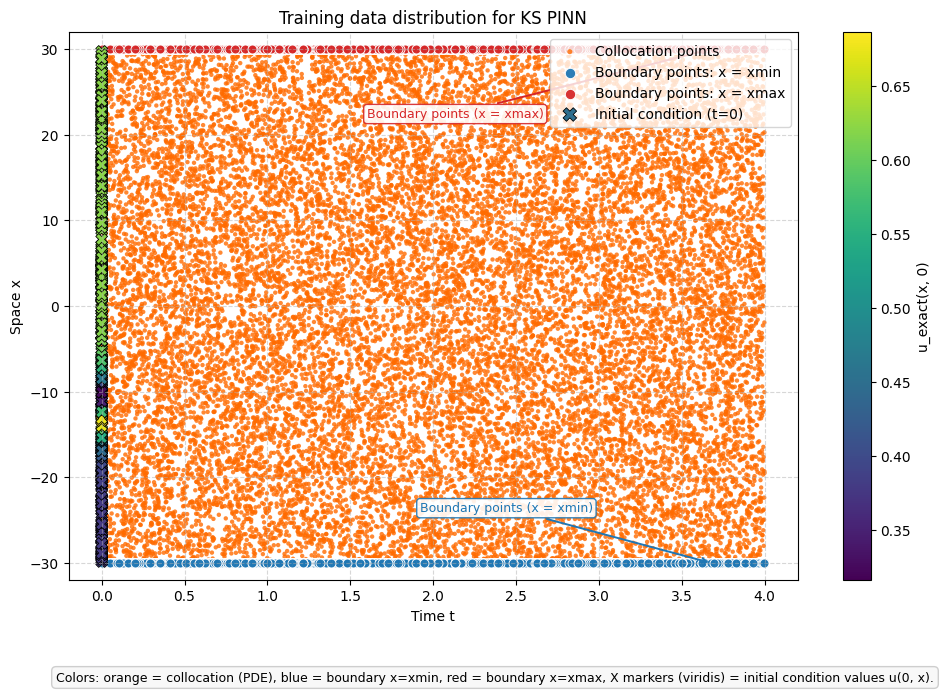
\includegraphics[width=0.8\linewidth]{stage_1/dataset.png}
    \caption{Обучающая выборка}
    \label{fig:dataset}
\end{figure}

Внутренние точки используются для минимизации невязки дифференциального уравнения, получаемой путём подстановки нейросетевой аппроксимации в исходное уравнение. Производные по пространственной и временной переменным, включая старшие производные, вычисляются с использованием автоматического дифференцирования.

Невязка уравнения имеет вид \cref{eq:pde-residual}:
\begin{equation}
\label{eq:pde-residual}
r_{\theta}(t,x) = \frac{\partial u_{\theta}}{\partial t} + u_{\theta}\frac{\partial u_{\theta}}{\partial x} + \frac{\partial^{2} u_{\theta}}{\partial x^2} + \frac{\partial^{4} u_{\theta}}{\partial x^4}.
\end{equation}

Функция потерь формируется как сумма нескольких слагаемых \cref{eq:loss-function,eq:loss-residual,eq:loss-initial,eq:loss-dirichlet,eq:loss-neumann}:
\begin{equation}
\label{eq:loss-function}
\mathcal{L} = \lambda_r \mathcal{L}_r + \lambda_0 \mathcal{L}_0 + \lambda_D \mathcal{L}_D + \lambda_N \mathcal{L}_N,
\end{equation}
где
\begin{equation}
\label{eq:loss-residual}
\mathcal{L}_r = \frac{1}{N_r} \sum_{i=1}^{N_r} \left| r_{\theta}(t_i,x_i) \right|^2,
\end{equation}
\begin{equation}
\label{eq:loss-initial}
\mathcal{L}_0 = \frac{1}{N_0} \sum_{i=1}^{N_0} \left| u_{\theta}(0,x_i) - u_0(x_i) \right|^2,
\end{equation}
\begin{equation}
\label{eq:loss-dirichlet}
\mathcal{L}_D = \frac{1}{N_b} \sum_{i=1}^{N_b} \left(
|u_{\theta}(t_i,-L) - u_1(t_i)|^2 + |u_{\theta}(t_i,L) - u_2(t_i)|^2
\right).
\end{equation}
\begin{equation}
\label{eq:loss-neumann}
\mathcal{L}_N = \frac{1}{N_b} \sum_{i=1}^{N_b} \left(
\left| \frac{\partial u_{\theta}}{\partial x}(t_i,-L) - u_3(t_i) \right|^2 +
\left| \frac{\partial u_{\theta}}{\partial x}(t_i,L) - u_4(t_i) \right|^2
\right).
\end{equation}

Здесь $N_r$, $N_0$, $N_b$ — количество внутренних, начальных и граничных точек соответственно, а $\lambda_r$, $\lambda_0$, $\lambda_D$, $\lambda_N$ — весовые коэффициенты.

Каждая из компонент в \cref{eq:loss-function} имеет самостоятельный физико-математический смысл. Слагаемое \cref{eq:loss-residual} отвечает за выполнение самого дифференциального уравнения во внутренних коллокационных точках области и тем самым обеспечивает физическую согласованность нейросетевой аппроксимации. Компонента \cref{eq:loss-initial} контролирует точность воспроизведения начального условия и заставляет сеть корректно восстанавливать профиль решения в момент времени $t=0$. Слагаемое \cref{eq:loss-dirichlet} штрафует отклонения значений $u_{\theta}(t,x)$ от заданных граничных условий Дирихле на концах пространственного интервала, то есть фиксирует значения решения на границе области. Наконец, компонента \cref{eq:loss-neumann} отвечает за выполнение граничных условий Неймана и согласует значения пространственной производной $\frac{\partial u_{\theta}}{\partial x}$ на границах с предписанными функциями $u_3(t)$ и $u_4(t)$. Таким образом, минимизация полной функции потерь означает одновременное стремление сети удовлетворить уравнению, начальному условию и обоим типам граничных ограничений, а весовые коэффициенты позволяют регулировать относительный вклад каждой из этих составляющих в процесс обучения.

Обучение сводится к задаче оптимизации \cref{eq:optimization}:
\begin{equation}
\label{eq:optimization}
\theta^* = \arg\min_{\theta} \mathcal{L}.
\end{equation}

С целью повышения качества восстановления решения в работе применяется нормирование искомой функции \cref{eq:normalization}:
\begin{equation}
\label{eq:normalization}
u(t,x) = u_s \cdot \tilde{u}(t,x),
\end{equation}
где $u_s$ — масштабный коэффициент.

Для рассматриваемой задачи важна корректная передача высокочастотных компонент и локальных перепадов решения. Однако классические полносвязные сети проявляют эффект спектрального смещения (spectral bias), то есть склонность сначала аппроксимировать низкочастотные составляющие \cite{rahaman2019spectral,tancik2020fourier}. Для ослабления этого эффекта входные переменные дополнительно преобразуются с помощью Фурье-кодирования \cref{eq:fourier-encoding}:
\begin{equation}
\label{eq:fourier-encoding}
\gamma(t) = [\sin(2\pi B_t t), \cos(2\pi B_t t)], \quad
\gamma(x) = [\sin(2\pi B_x x), \cos(2\pi B_x x)].
\end{equation}

Конкретные параметры вычислительного эксперимента, пространственно-временная область, длительность обучения и детали сравнения с точным решением приведены в главе 2.


\section{Этап 1: базовый вычислительный эксперимент}

\subsection{Формирование обучающего множества и коллокация}

Вычислительный эксперимент для решения уравнения Курамото–Сивашинского проводился в прямоугольной пространственно-временной области $(t,x) \in [0, 4] \times [-30, 30]$. Обучающее множество строилось по общей схеме, описанной в разделе 1.2: точки начального условия задавались на слое $t=0$, точки граничных условий --- на границах $x=-30$ и $x=30$, а внутренние коллокационные точки распределялись внутри всей области. Во всех трёх группах использовалось случайное равномерное распределение в соответствующих подмножествах области определения. Схематически распределение точек показано на \cref{fig:dataset}.

\subsection{Параметры базовой модели}

В качестве базовой модели использовалась полносвязная нейронная сеть $u_\theta(t,x)$ с нормированием выходной переменной и Фурье-кодированием входов, введёнными в разделе 1.2. Такое сочетание позволяло стабилизировать масштаб выходной функции и повысить способность сети передавать локальные пространственные особенности точного решения.

Обучение базовой модели проводилось до $13000$ эпох. Для анализа динамики сходимости и эволюции аппроксимации дополнительно рассматривались промежуточные состояния после $3000$, $7000$ и $10000$ эпох. Качество восстановления оценивалось сравнением с точным аналитическим решением на характерных временных срезах $t=0$ и $t=4$.

\subsection{Анализ динамики обучения и эволюция аппроксимации}

Графики \cref{fig:stage1_aprox1,fig:stage1_aprox3,fig:stage1_aprox7,fig:stage1_aprox13,fig:stage1_aprox14} показывают типичную для PINN последовательность этапов обучения. На начальной стадии предсказание остаётся сглаженным и существенно отличается от точного решения как по амплитуде, так и по положению фронта. Такое поведение согласуется с доминированием residual-компоненты, содержащей производную четвёртого порядка: на ранних итерациях сеть предпочитает низкочастотные профили с малой кривизной.
 
\begin{figure}[ht!]
    \centering
    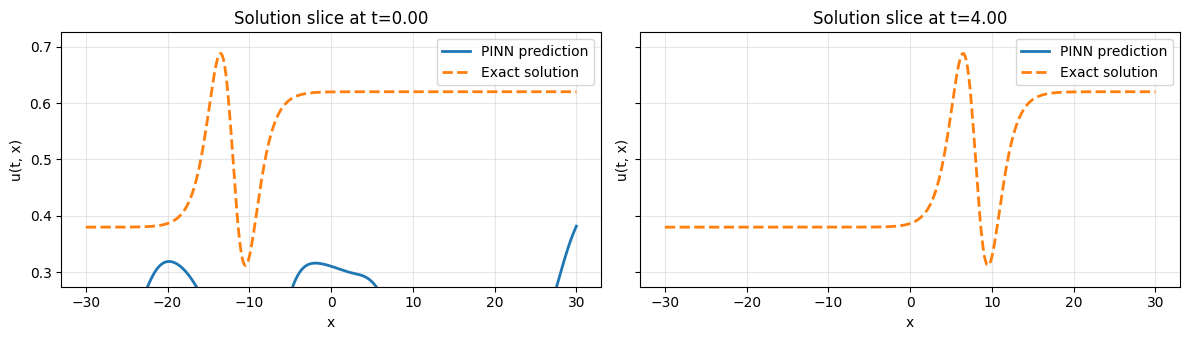
\includegraphics[width=0.8\linewidth]{stage_1/aprox1.png}
    \caption{Начальная эпоха}
    \label{fig:stage1_aprox1}
\end{figure}

На промежуточных итерациях модель начинает воспроизводить глобальную геометрию бегущей волны: формируются основной пик и следующая за ним впадина, уменьшается ошибка на срезе $t=0$, а профиль при $t=4$ приобретает корректное направление переноса. В то же время сохраняются фазовый сдвиг и ошибка амплитуды, что указывает на неполное согласование между выполнением уравнения и воспроизведением временной эволюции решения.

\begin{figure}[ht!]
    \centering
    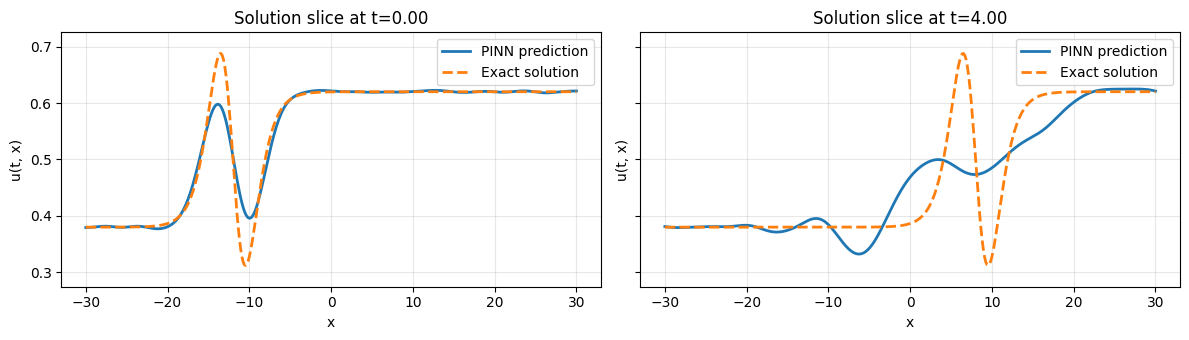
\includegraphics[width=0.8\linewidth]{stage_1/aprox3.png}
    \caption{3000-я эпоха}
    \label{fig:stage1_aprox3}

\end{figure}
\begin{figure}[ht!]
    \centering
    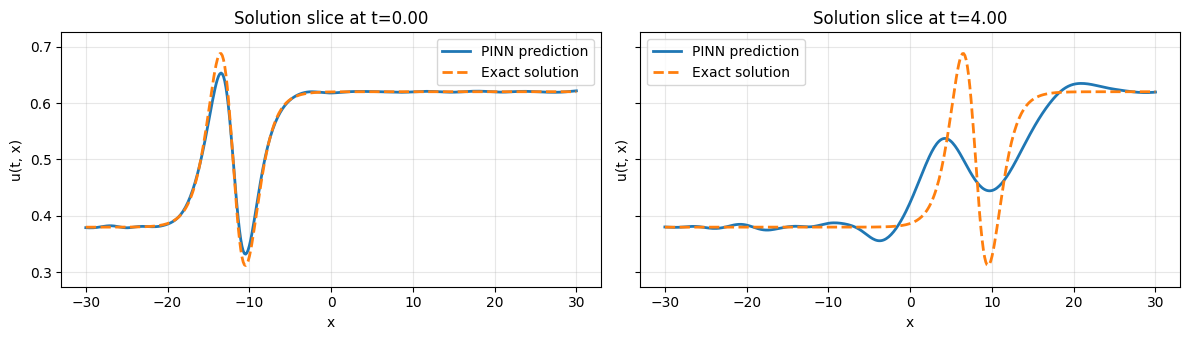
\includegraphics[width=0.8\linewidth]{stage_1/aprox7.png}
    \caption{7000-я эпоха}
    \label{fig:stage1_aprox7}

\end{figure}
\begin{figure}[ht!]
    \centering
    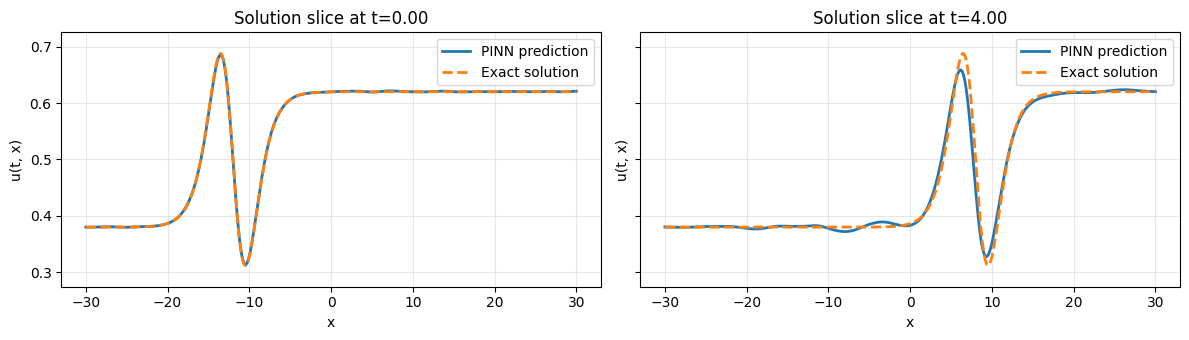
\includegraphics[width=0.8\linewidth]{stage_1/aprox13.png}
    \caption{10000-я эпоха}
    \label{fig:stage1_aprox13}
\end{figure}

На заключительной стадии предсказание практически совпадает с точным решением на рассматриваемых временных срезах. Модель корректно воспроизводит нелинейный профиль типа $\tanh/\tanh^3$, пространственный сдвиг волны и масштаб амплитуды.
\begin{figure}[ht!]
    \centering
    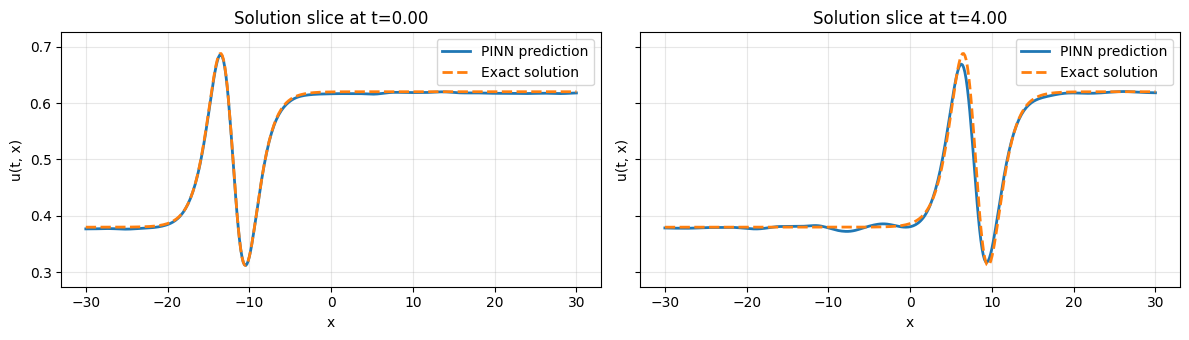
\includegraphics[width=0.8\linewidth]{stage_1/aprox14.png}
    \caption{13000-я эпоха}
    \label{fig:stage1_aprox14}
\end{figure}

\subsection{Анализ ошибки}
Как показывает \cref{fig:lossComponets}, компоненты функции потерь убывают с различной скоростью. На ранних итерациях ошибка по начальному условию снижается быстрее, чем ошибка, связанная с граничными ограничениями. На поздней стадии компонент, соответствующий условиям Неймана, демонстрирует более ровную динамику и меньшую чувствительность к высокочастотным колебаниям, чем ошибка по начальному условию. В пределах данного эксперимента его можно рассматривать как более устойчивый ориентир при анализе сходимости отдельных частей функционала.

\begin{figure}[ht!]
\centering
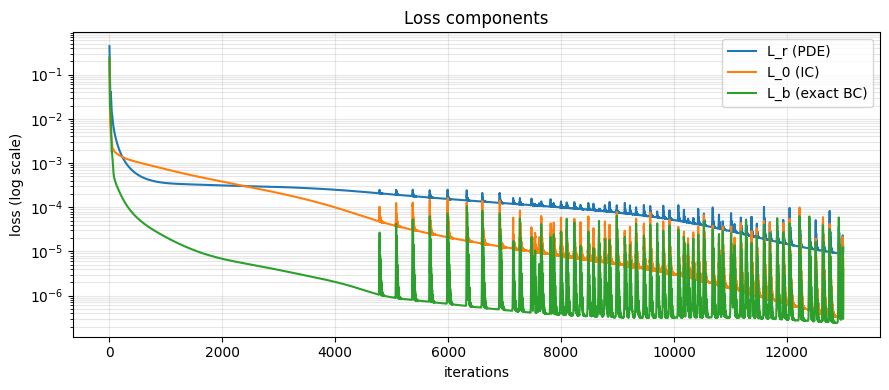
\includegraphics[width=0.8\linewidth]{stage_1/lossComponets.png}
\caption{Динамика компонент функции потерь, соответствующих различным условиям задачи}
\label{fig:lossComponets}
\end{figure}

Суммарная функция потерь (\cref{fig:total_loss}) в целом демонстрирует хорошую сходимость: значение ошибки монотонно убывает на протяжении большей части процесса обучения и достигает порядка $10^{-5}$, что соответствует качественной аппроксимации.
На заключительном участке появляются локальные осцилляции, согласующиеся с ростом вклада одной из граничных компонент. Это указывает на дисбаланс между отдельными частями функционала и делает оправданным дополнительное перевзвешивание условий в функции потерь.


\begin{figure}[ht!]
\centering
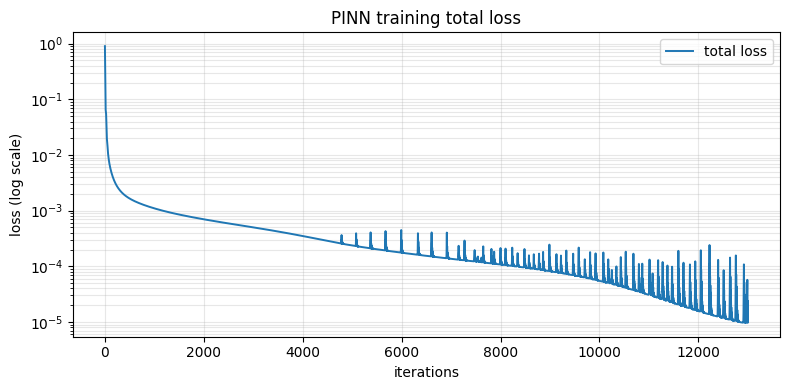
\includegraphics[width=0.8\linewidth]{stage_1/total_loss.png}
\caption{Динамика суммарной функции потерь}
\label{fig:total_loss}
\end{figure}

\section{Этап 2: понижение порядка и анализ деградации точности}
\subsection{Модификация постановки задачи и варианты архитектур PINN}

На втором этапе проверялась гипотеза о том, что понижение порядка старшей пространственной производной может упростить обучение PINN. Для этого была введена дополнительная вспомогательная переменная \cref{eq:auxiliary-variable}:
\begin{equation}
\label{eq:auxiliary-variable}
v = \frac{\partial^2 u}{\partial x^2}
\end{equation}

Данная подстановка преобразует исходное уравнение с производными четвёртого порядка в систему уравнений не выше второго порядка, задаваемую \cref{eq:reduced-pde,eq:compatibility-condition}:
\begin{equation}
\label{eq:reduced-pde}
\frac{\partial u}{\partial t} + u \frac{\partial u}{\partial x} + v + \frac{\partial^2 v}{\partial x^2} = 0.
\end{equation}
\begin{equation}
\label{eq:compatibility-condition}
v - \frac{\partial^2 u}{\partial x^2} = 0.
\end{equation}
Мотивацией такой замены было исключение прямого вычисления производной четвёртого порядка, которое в PINN часто сопровождается жёсткостью градиентов и повышенной чувствительностью к гиперпараметрам. Вместе с тем новая постановка не сводится к упрощению оптимизации: она вводит дополнительное поле $v(t,x)$ и условие согласования \cref{eq:compatibility-condition}, так что сеть должна одновременно восстановить $u(t,x)$, $v(t,x)$ и их взаимосвязь во всей области.

Для решения модифицированной системы были рассмотрены три архитектуры:
\begin{itemize}
    \item \textbf{Единая нейронная сеть с двумя выходами (\texttt{two\_output}):} Отображение пространства входов в двумерный выход $(u, v)$ с общим скрытым представлением.
    \item \textbf{Две независимые нейронные сети (\texttt{two\_models}):} Полное разделение параметров, где функции $u$ и $v$ аппроксимируются изолированными сетями.
    \item \textbf{Сеть с общим стволом и раздельными ветвями (\texttt{shared\_trunk}):} Гибридный подход, при котором начальные слои извлекают общие физические закономерности, а независимые «головы» адаптируются к спецификам $u$ и $v$.
\end{itemize}

\subsection{Динамика обучения и сравнительный анализ архитектур}

На \cref{fig:stage_2_all_error} для всех архитектур второго этапа наблюдается одна и та же закономерность. На начальных итерациях total loss быстро убывает, затем после примерно $3 \cdot 10^3$--$4 \cdot 10^3$ шагов темп сходимости резко снижается, и траектории переходят в режим плато. Финальные значения total loss стабилизируются на уровне $1.4 \cdot 10^{-4} - 1.5 \cdot 10^{-4}$, тогда как базовая модель первого этапа достигает уровня порядка $10^{-5}$. Следовательно, понижение порядка производной не устранило оптимизационный барьер, а перенесло его в новую постановку.

\begin{figure}[ht!]
\centering
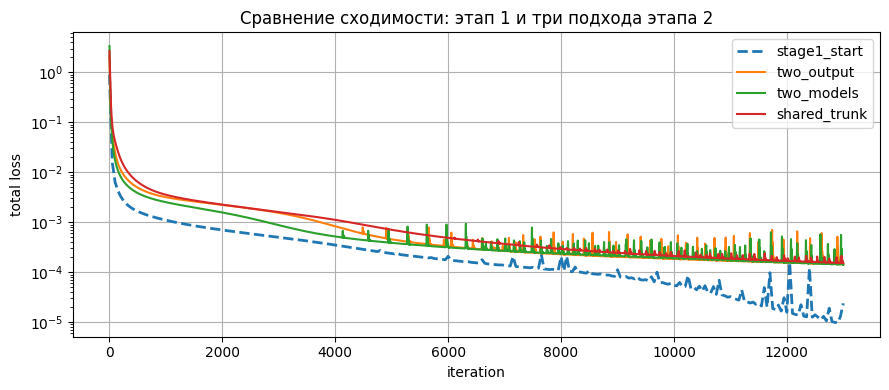
\includegraphics[width=0.8\linewidth]{stage_2/all_error.png}
\caption{Сравнение ошибок аппроксимации четырёх моделей}
\label{fig:stage_2_all_error}
\end{figure}
\FloatBarrier

Сравнение кривых total loss на \cref{fig:stage_2/shared_trunk_total_loss,fig:stage_2/tow_output_total_loss,fig:stage_2_tow_model_total_loss} показывает, что среди архитектур второго этапа наиболее ровную траекторию и наименьший финальный уровень ошибки демонстрирует \texttt{shared\_trunk}. Архитектура \texttt{two\_output} близка к ней по уровню ошибки, но сохраняет более регулярные всплески. Наиболее выраженные осцилляции наблюдаются у \texttt{two\_models}, что указывает на наименьшую устойчивость этой схемы.

\begin{figure}[ht!]
\centering
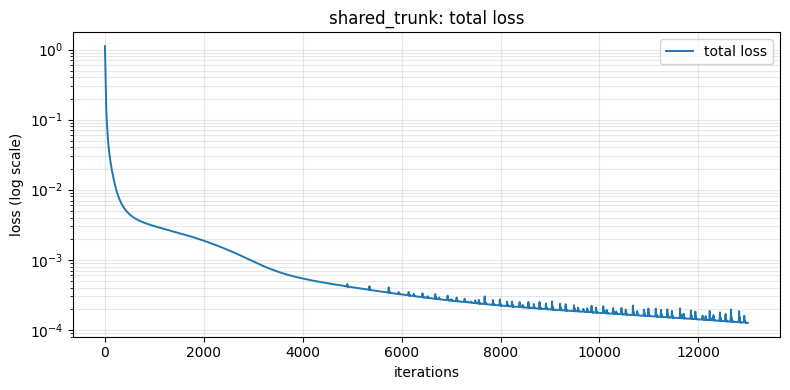
\includegraphics[width=0.8\linewidth]{stage_2/shared_trunk_total_loss.png}
\caption{Общая ошибка гибридной модели с общим стволом}
\label{fig:stage_2/shared_trunk_total_loss}
\end{figure}

\begin{figure}[ht!]
\centering
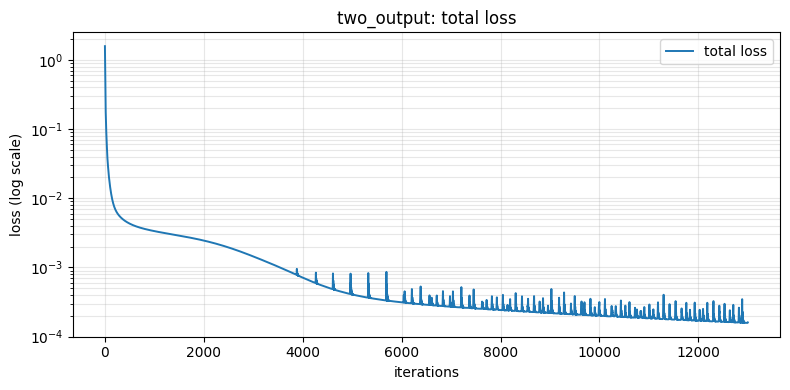
\includegraphics[width=0.8\linewidth]{stage_2/tow_output_total_loss.png}
\caption{Общая ошибка модели с двумя выходами}
\label{fig:stage_2/tow_output_total_loss}
\end{figure}

\begin{figure}[ht!]
\centering
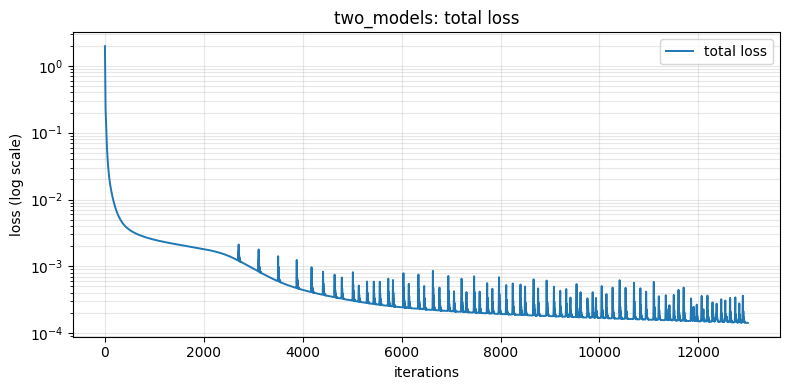
\includegraphics[width=0.8\linewidth]{stage_2/tow_model_total_loss.png}
\caption{Общая ошибка модели с двумя независимыми нейронными сетями}
\label{fig:stage_2_tow_model_total_loss}
\end{figure}

Графики компонент функции потерь на \cref{fig:stage_2/shared_trunk_loss_components,fig:stage_2/tow_model_loss_components,fig:stage_2/tow_output_loss_components} показывают, что во всех трёх случаях ключевым ограничением остаётся невязка уравнения $L_r$. Компоненты начального условия $L_0$ и граничных условий $L_b$ убывают быстрее и к концу обучения оказываются на один--два порядка ниже. Тем самым общая закономерность обучения моделей второго этапа состоит в следующем: начальное снижение total loss достигается за счёт быстрого уменьшения ошибок по данным и граничным ограничениям, после чего дальнейшая сходимость определяется residual-компонентой и необходимостью согласования полей $u$ и $v$.

\begin{figure}[ht!]
\centering
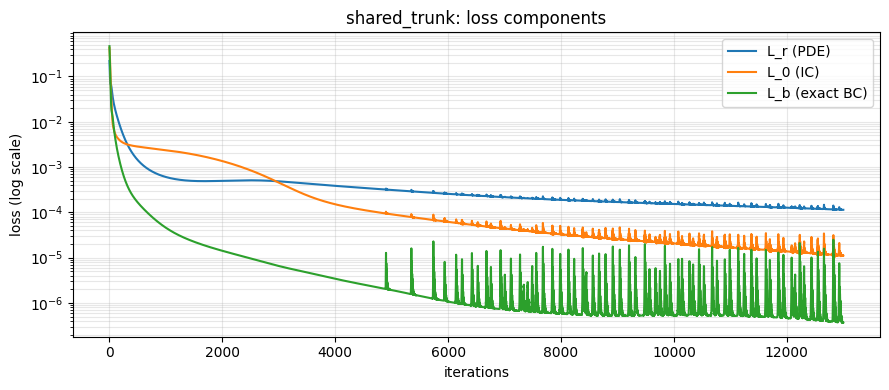
\includegraphics[width=0.8\linewidth]{stage_2/shared_trunk_loss_components.png}
\caption{Компоненты функции потерь гибридной модели с общим стволом}
\label{fig:stage_2/shared_trunk_loss_components}
\end{figure}

\begin{figure}[ht!]
\centering
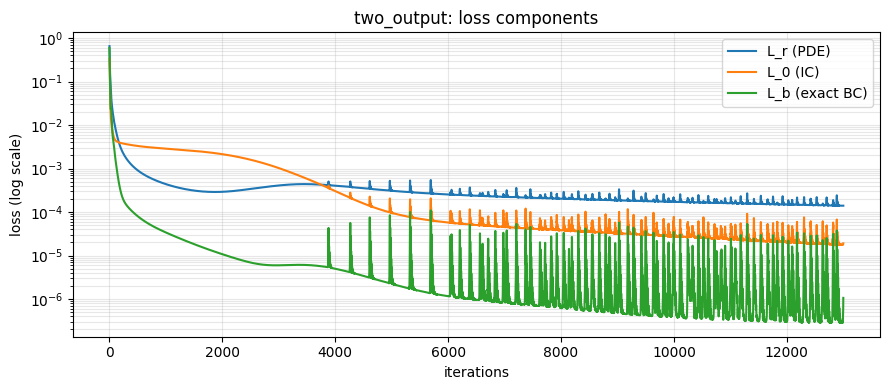
\includegraphics[width=0.8\linewidth]{stage_2/tow_output_loss_components.png}
\caption{Компоненты функции потерь модели с двумя выходами}
\label{fig:stage_2/tow_output_loss_components}
\end{figure}

\begin{figure}[ht!]
\centering
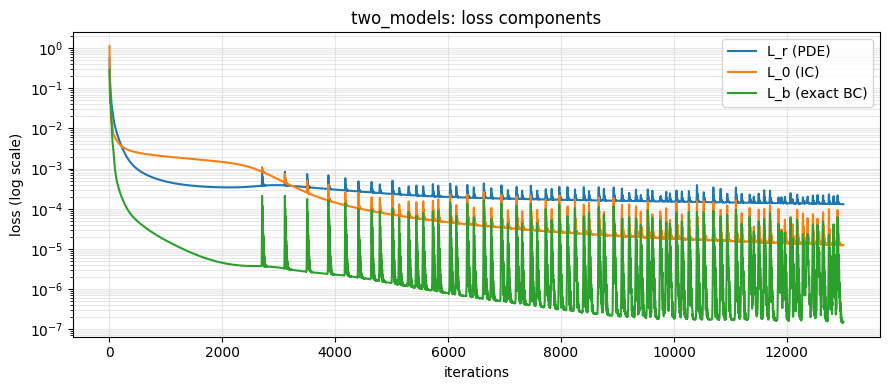
\includegraphics[width=0.8\linewidth]{stage_2/tow_model_loss_components.png}
\caption{Компоненты функции потерь модели с двумя независимыми нейронными сетями}
\label{fig:stage_2/tow_model_loss_components}
\end{figure}

Пики на кривых total loss и отдельных компонент возникают при попытках дальнейшего уменьшения $L_r$ после выхода на плато. Их наибольшая амплитуда в \texttt{two\_models} согласуется с тем, что две независимые сети должны синхронизироваться только через функционал потерь. В \texttt{two\_output} этот конфликт выражен слабее, однако общее скрытое представление должно одновременно кодировать поля разной гладкости и масштаба. В \texttt{shared\_trunk} общие пространственно-временные признаки извлекаются совместно, а различия между $u$ и $v$ частично компенсируются раздельными выходными ветвями, что соответствует более ровкой динамике.

\FloatBarrier

Эволюция аппроксимации на \cref{fig:stage_2/shared_trunk_aprox_evalution,fig:stage_2/tow_output_aprox_evolution,fig:stage_2/tow_model_aprox_evalution} показывает, что во всех архитектурах поле $u(t,x)$ восстанавливается заметно лучше, чем поле $v(t,x)$. На срезе $t=0$ все три модели после обучения передают основную структуру фронта. На срезах $t=2$ и $t=4$ различия становятся более выраженными: \texttt{shared\_trunk} лучше сохраняет положение фронта и амплитуду, \texttt{two\_output} занимает промежуточное положение, а \texttt{two\_models} демонстрирует наиболее заметное сглаживание переходных зон.

Для поля $v(t,x)$ ни одна из архитектур не воспроизводит с той же точностью узкие знакопеременные пики точного решения на поздних временных срезах. Предсказания остаются сглаженными и имеют заниженную амплитуду, что указывает на трудности восстановления локальной кривизны, связанной с условием $v=u_{xx}$. Та же закономерность отражается и на сводном графике ошибки: минимальную относительную ошибку среди архитектур второго этапа демонстрирует \texttt{shared\_trunk}, за ним следует \texttt{two\_output}, тогда как \texttt{two\_models} показывает наихудший результат.

\begin{figure}[ht!]
\centering
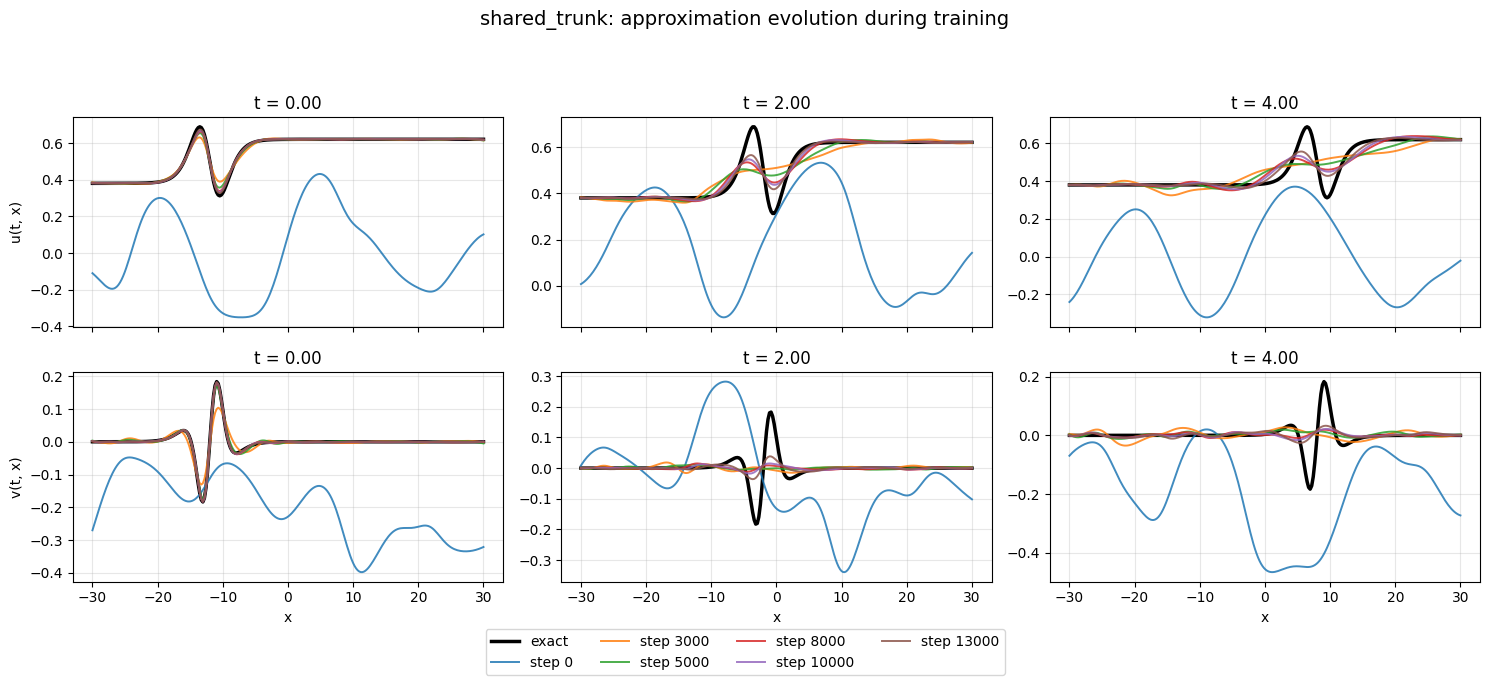
\includegraphics[width=1\linewidth]{stage_2/shared_trunk_aprox_evalution.png}
\caption{Эволюция аппроксимации гибридной модели с общим стволом}
\label{fig:stage_2/shared_trunk_aprox_evalution}
\end{figure}

\begin{figure}[ht!]
\centering
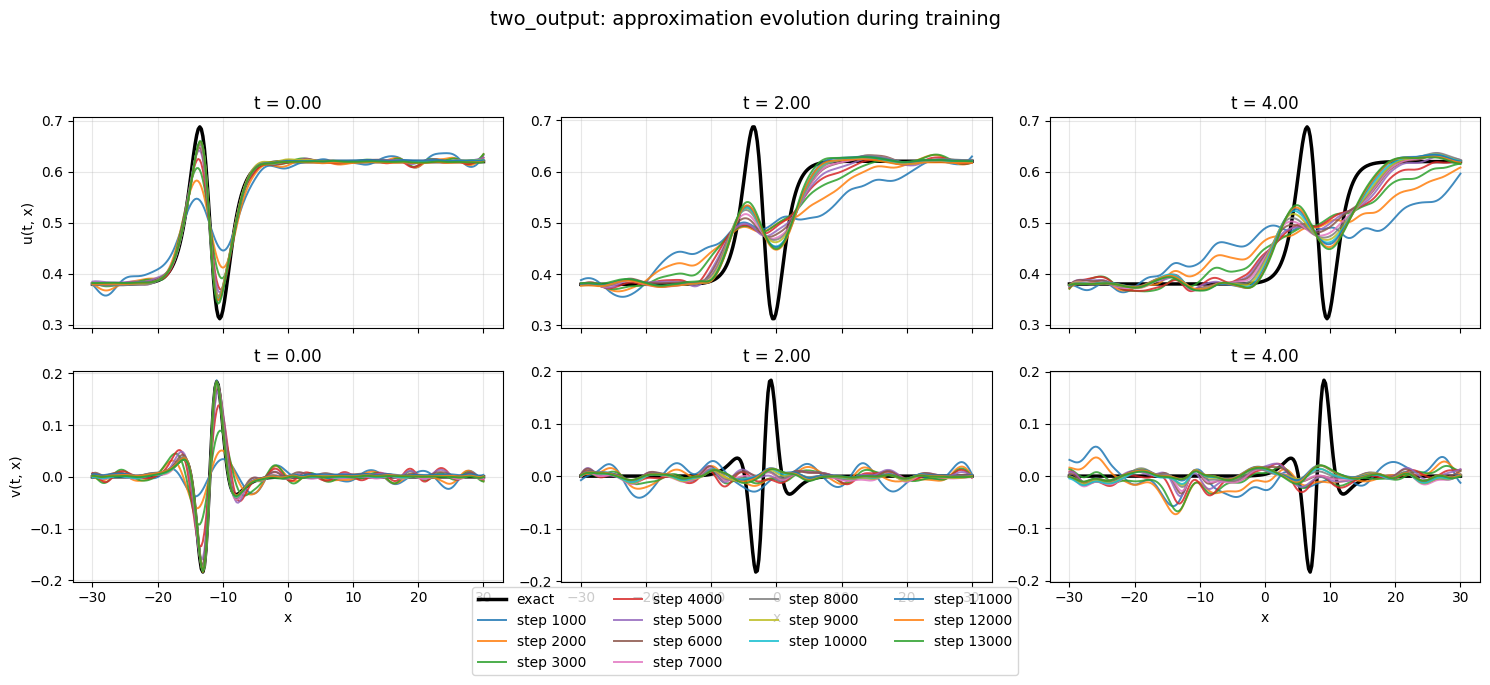
\includegraphics[width=1\linewidth]{stage_2/tow_output_aprox_evolution.png}
\caption{Эволюция аппроксимации модели с двумя выходами}
\label{fig:stage_2/tow_output_aprox_evolution}
\end{figure}

\begin{figure}[ht!]
\centering
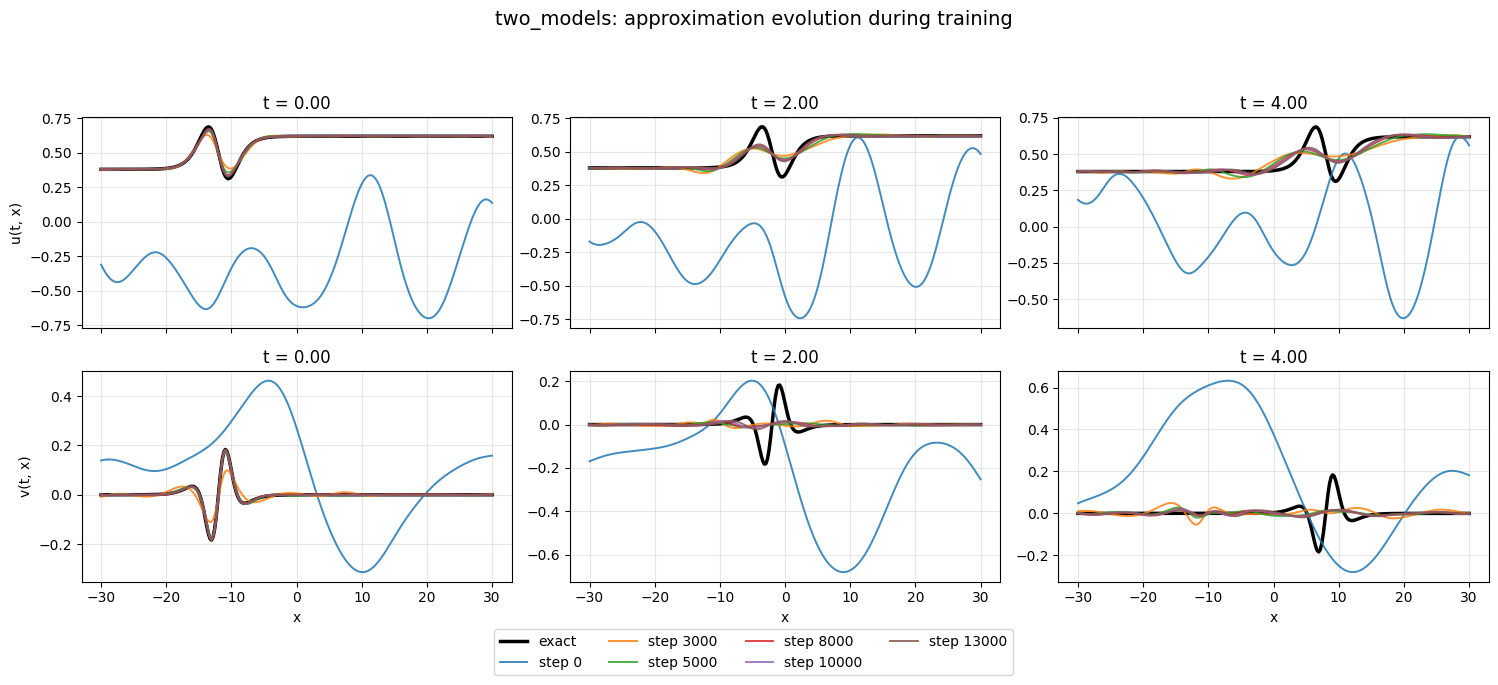
\includegraphics[width=1\linewidth]{stage_2/tow_model_aprox_evalution.png}
\caption{Эволюция аппроксимации модели с двумя независимыми нейронными сетями}
\label{fig:stage_2/tow_model_aprox_evalution}
\end{figure}


\subsection{Причины деградации точности}

Наблюдаемая деградация точности связана со структурой новой задачи оптимизации. Понижение порядка производной устраняет прямое вычисление $u_{xxxx}$, но заменяет его одновременным обучением двух полей с различной гладкостью. Поле $u(t,x)$ задаёт сравнительно гладкий бегущий фронт, тогда как $v(t,x)=u_{xx}(t,x)$ содержит более локальные и знакопеременные структуры. Поэтому малое локальное отклонение в $u$ усиливается как в аппроксимации $v$, так и в невязке условия согласования \cref{eq:compatibility-condition}.

Эта структура согласуется с общей динамикой обучения. На ранней стадии уменьшение total loss обеспечивается главным образом за счёт снижения ошибок по начальному и граничным условиям и за счёт восстановления грубой формы поля $u$. После этого дальнейшее уменьшение ошибки требует одновременного снижения residual-компоненты и невязки согласования между $u$ и $v$, что и приводит к формированию плато.

Архитектурные различия определяются тем, как каждая схема разрешает эту многомасштабную связь. В \texttt{two\_models} взаимодействие между $u$ и $v$ реализуется только через функционал потерь, поэтому обновление одной сети меняет целевую конфигурацию для другой; это соответствует наиболее выраженным осцилляциям. В \texttt{two\_output} конфликт ослаблен общим скрытым представлением, но оно должно одновременно кодировать поля разного масштаба. Архитектура \texttt{shared\_trunk} обеспечивает компромисс между совместным извлечением общих признаков и специализацией выходов, что согласуется с меньшей амплитудой колебаний и более низкой итоговой ошибкой \cite{wang2021gradient,wang2022ntk}.

\subsection{Выводы: деградация эффективности при усложнении системы}

Результаты второго этапа допускают три основных вывода:
\begin{enumerate}
    \item Для всех архитектур второго этапа характерно быстрое начальное снижение total loss, после которого обучение переходит в режим плато. Лимитирующим фактором при этом становится residual-компонента и связанное с ней согласование полей $u$ и $v$.
    \item Понижение порядка за счёт введения переменной $v$ не привело к улучшению точности по сравнению с прямой аппроксимацией исходного уравнения четвёртого порядка. Финальные ошибки моделей второго этапа остаются примерно на порядок выше, чем у базовой модели первого этапа.
    \item Среди рассмотренных архитектур наименьшую итоговую ошибку и наиболее устойчивую динамику обучения демонстрирует \texttt{shared\_trunk}; архитектура \texttt{two\_output} занимает промежуточное положение, а \texttt{two\_models} оказывается наименее устойчивой.
\end{enumerate}

С учётом наблюдаемого дисбаланса между компонентами функции потерь для данной постановки оправдано адаптивное перевзвешивание residual- и boundary-компонент, а также раздельное масштабирование выходов $u$ и $v$.

\section{Анализ Neural Tangent Kernel для сети 1 первого этапа }

\subsection{Описание нейронного косательного ядра }

Neural Tangent Kernel (NTK) представляет собой ядро, порожденное нейронной сетью через градиенты выхода сети по её параметрам. В современной теории глубокого обучения NTK играет важную роль, поскольку позволяет описывать обучение нейронной сети в функциональном пространстве, а не только в пространстве параметров. Это особенно важно в режиме большой ширины, когда динамика градиентного спуска приобретает почти линейный характер и становится близкой к обучению ядрового метода.

Ключевая идея состоит в том, что при достаточно большой ширине скрытых слоёв случайно инициализированная сеть ведёт себя почти как линейная модель относительно параметров в окрестности точки инициализации. В этом пределе NTK стремится к детерминированному ядру, а обучение сети по градиентному спуску оказывается эквивалентным kernel regression с данным ядром. Поэтому NTK служит мостом между теорией глубоких сетей, гауссовскими процессами и классическими ядровыми методами.

\subsection{Математическое обоснование}

\subsubsection{Определение NTK}

Пусть нейронная сеть задаёт скалярную функцию
\begin{equation}
    f(x,\theta): \mathbb{R}^d \to \mathbb{R},
\end{equation}
где $x$ --- вход, а $\theta \in \mathbb{R}^p$ --- вектор параметров сети. Для двух входов $x$ и $x'$ Neural Tangent Kernel определяется как скалярное произведение градиентов выхода сети по параметрам:
\begin{equation}
    K(x,x';\theta)=\nabla_{\theta} f(x,\theta)^{\top}\nabla_{\theta} f(x',\theta).
    \label{eq:ntk_def}
\end{equation}

Если рассматривать набор точек $X=\{x_i\}_{i=1}^{n}$, то соответствующая матрица NTK имеет вид
\begin{equation}
    \Theta_{ij}(\theta)=K(x_i,x_j;\theta)=\nabla_{\theta} f(x_i,\theta)^{\top}\nabla_{\theta} f(x_j,\theta).
    \label{eq:ntk_matrix}
\end{equation}

Иначе говоря, NTK измеряет сходство двух входов не в исходном пространстве признаков, а в пространстве чувствительности модели к своим параметрам.

\subsubsection{Переход к линейной динамике обучения}

Рассмотрим обучение по функции потерь среднеквадратичного отклонения
\begin{equation}
    \mathcal{L}(\theta)=\frac{1}{2}\sum_{i=1}^{n}\bigl(f(x_i,\theta)-y_i\bigr)^2.
\end{equation}
В режиме непрерывного времени градиентный спуск записывается как gradient flow:
\begin{equation}
    \frac{d\theta}{dt}=-\nabla_{\theta}\mathcal{L}(\theta)
    =-\sum_{j=1}^{n}\bigl(f(x_j,\theta)-y_j\bigr)\nabla_{\theta}f(x_j,\theta).
    \label{eq:gradient_flow_theta}
\end{equation}

Обозначим через
\begin{equation}
    u_i(t)=f(x_i,\theta(t)), \qquad u(t)=\bigl(u_1(t),\dots,u_n(t)\bigr)^{\top}.
\end{equation}
Тогда по правилу цепочки
\begin{equation}
    \frac{du_i}{dt}
    =\nabla_{\theta}f(x_i,\theta)^{\top}\frac{d\theta}{dt}.
\end{equation}
Подставляя \eqref{eq:gradient_flow_theta}, получаем
\begin{equation}
    \frac{du_i}{dt}
    =-\sum_{j=1}^{n}\Theta_{ij}(\theta)\bigl(u_j(t)-y_j\bigr).
\end{equation}
В матричной форме это даёт
\begin{equation}
    \frac{du}{dt}=-\Theta(\theta(t))\bigl(u(t)-y\bigr).
    \label{eq:functional_dynamics}
\end{equation}

Формула \eqref{eq:functional_dynamics} показывает, что именно матрица NTK определяет скорость уменьшения ошибки по различным направлениям в пространстве функций. Если в ходе обучения ядро меняется мало, то можно считать
\begin{equation}
    \Theta(\theta(t))\approx \Theta(\theta_0)=\Theta_0,
\end{equation}
и тогда динамика становится линейной:
\begin{equation}
    \frac{du}{dt}=-\Theta_0\bigl(u(t)-y\bigr).
\end{equation}
Решение этой системы имеет вид
\begin{equation}
    u(t)-y=\exp(-\Theta_0 t)\bigl(u(0)-y\bigr).
    \label{eq:matrix_exp_solution}
\end{equation}

Таким образом, компоненты ошибки, соответствующие большим собственным значениям NTK, затухают быстрее, тогда как направления, связанные с малыми собственными значениями, обучаются медленнее.

\subsubsection{Связь  регрессией и динамика NTK в пределе бесконечной ширины}

В режиме линеаризованного (так называемого «ленивого») обучения динамика нейронной сети большой ширины аналитически эквивалентна методам ядерной регрессии. Если процесс оптимизации продолжается до полной интерполяции данных обучающей выборки при условии квазистационарности NTK, предельное решение для произвольного входного вектора $x$ принимает следующую форму:
\begin{equation}
    f_{\infty}(x) = f_0(x) + \Theta(x, X) \Theta(X, X)^{-1} \bigl(y - f_0(X)\bigr),
    \label{eq:kernel_regression_ntk}
\end{equation}
где $f_0$ — аппроксимирующая функция в момент случайной инициализации параметров, $\Theta(x, X)$ — вектор значений NTK между точкой $x$ и объектами обучающей выборки, а $\Theta(X, X)$ — матрица Грама NTK.

Матрица Грама $\Theta(X, X) \in \mathbb{R}^{N \times N}$ представляет собой симметричную положительно полуопределенную матрицу, где $N$ — количество обучающих примеров. Каждый её элемент $(i, j)$ определяется как скалярное произведение градиентов выхода сети по вектору параметров $\theta$, вычисленных в точках $x_i$ и $x_j$:
\begin{equation}
    \Theta_{ij} = \langle \nabla_{\theta} f(x_i, \theta), \nabla_{\theta} f(x_j, \theta) \rangle.
\end{equation}
Визуально матрица Грама характеризует геометрию признакового пространства, порожденное архитектурой сети: диагональные элементы отражают «чувствительность» сети к отдельным объектам, а внедиагональные — степень информационного перекрытия и взаимного влияния пар объектов при обновлении параметров.

Устойчивость NTK при увеличении ширины слоёв $m \to \infty$ обосновывается законом больших чисел. Поскольку вклад каждого отдельного нейрона в итоговый результат становится исчезающе малым, совокупная матрица NTK при инициализации концентрируется около своего детерминированного предела:
\begin{equation}
    \Theta(\theta_0) \xrightarrow[m\to\infty]{} \Theta_{\infty}.
\end{equation}
При выборе адекватной параметризации изменения параметров в процессе обучения имеют порядок, недостаточный для значимого изменения ядра. Следовательно, на конечном временном интервале выполняется приближенное равенство $\Theta(\theta(t)) \approx \Theta_{\infty}$, что обуславливает переход динамики системы в режим, близкий к линейному.

С содержательной точки зрения NTK служит мерой подобия откликов сети. Если градиенты $\nabla_{\theta} f(x, \theta)$ и $\nabla_{\theta} f(x', \theta)$ характеризуются высокой степенью сонаправленности, то минимизация ошибки в точке $x$ приведет к синхронному изменению предсказания в точке $x'$. Таким образом, NTK можно интерпретировать как оператор распространения информации, определяющий, как локальное исправление ошибки на одном объекте транслируется на всю выборку.
\subsection{Спектральные и алгебраические свойства NTK}

Матрица NTK обладает рядом фундаментальных свойств, определяющих характер оптимизации и обобщающую способность нейронных сетей в режиме бесконечной ширины.



На основе аналитического определения NTK как скалярного произведения градиентов функции по параметрам, матрица $\Theta(X,X)$ для любой конечной выборки $X=\{x_i\}_{i=1}^{n}$ является симметричной и положительно полуопределенной. Свойство симметричности $K(x,x';\theta)=K(x',x;\theta)$ следует из коммутативности скалярного произведения. Положительная полуопределенность подтверждается анализом квадратичной формы для произвольного вектора коэффициентов $c \in \mathbb{R}^n$:
\begin{equation}
    c^{\top}\Theta c
    =\sum_{i,j=1}^{n}c_i c_j \nabla_{\theta}f(x_i,\theta)^{\top}\nabla_{\theta}f(x_j,\theta)
    =\left\|\sum_{i=1}^{n} c_i \nabla_{\theta}f(x_i,\theta)\right\|_2^2 \ge 0.
\end{equation}
Из этого следует, что в условиях точной арифметики все собственные значения $\lambda_i$ матрицы NTK неотрицательны. Появление незначительных отрицательных значений в практических численных экспериментах обычно интерпретируется как следствие погрешностей машинного округления.

Спектральное разложение матрицы $\Theta = Q \Lambda Q^{\top}$ (где $\Lambda=\mathrm{diag}(\lambda_1,\dots,\lambda_n)$ и $\lambda_1 \ge \lambda_2 \ge \dots \ge 0$) позволяет оценить количество независимых направлений изменения аппроксимирующей функции. Скорость диссипации (затухания) спектра определяет эффективную сложность модели: быстрое убывание собственных значений указывает на доминирование низкоразмерного подпространства в процессе обучения. Для количественного описания структуры матрицы используются след ($\mathrm{trace}(\Theta)$), ранг ($\mathrm{rank}(\Theta)$) и эффективный ранг ($r_{\mathrm{eff}}$), вычисляемый через энтропию нормированного спектра:
\begin{equation}
    p_i=\frac{\lambda_i}{\sum_j \lambda_j}, \qquad
    r_{\mathrm{eff}}=\exp\left(-\sum_i p_i \ln p_i\right).
\end{equation}
Эффективный ранг служит мерой информационной емкости модели, отражая реальное число степеней свободы, задействованных при подгонке данных.

\subsubsection{Обусловленность и устойчивость динамики}

Важнейшим дескриптором устойчивости процесса обучения является число обусловленности, определяемое как отношение максимального собственного значения к минимальному положительному:
\begin{equation}
    \kappa(\Theta)=\frac{\lambda_{\max}}{\lambda_{\min}^{+}}.
\end{equation}
Высокое значение $\kappa(\Theta)$ свидетельствует о плохой обусловленности системы, что влечет за собой существенную неоднородность скоростей сходимости: компоненты ошибки, соответствующие старшим собственным числам, подавляются экспоненциально быстро, в то время как компоненты, связанные с хвостом спектра, требуют длительного времени для коррекции. Такая «жесткая» динамика повышает чувствительность модели к шумовым компонентам выборки и снижает стабильность численных алгоритмов оптимизации.
\subsection{Практический пример: вычисление NTK для MLP в TensorFlow}

Для практической демонстрации рассмотрим полносвязную сеть (MLP) с двумя скрытыми слоями и нелинейностью $\tanh$. На конечной выборке $\{x_i\}_{i=1}^{n}$ эмпирический NTK вычисляется следующим образом:
\begin{enumerate}
    \item для каждого входа $x_i$ вычисляется градиент $\nabla_{\theta} f(x_i,\theta)$;
    \item градиенты векторизуются и собираются в матрицу Якоби $J \in \mathbb{R}^{n \times p}$;
    \item матрица NTK строится как
    \begin{equation}
        \Theta = J J^{\top}.
    \end{equation}
\end{enumerate}

В данной работе все вычисления проводились в \texttt{TensorFlow}. Для фиксированной выборки эмпирическая матрица NTK строилась как на инициализации, так и после завершения обучения MLP, после чего по ней вычислялись спектр собственных значений, ранг, effective rank и condition number. На основе этих данных были получены тепловые карты NTK до и после обучения, PCA-проекция строк матрицы и кластеризованная матрица, что позволило сопоставить спектральные характеристики ядра с геометрией данных и с наблюдаемой динамикой оптимизации.

\subsection{Визуализации и анализ результатов}

\begin{figure}[ht!]
    \centering
    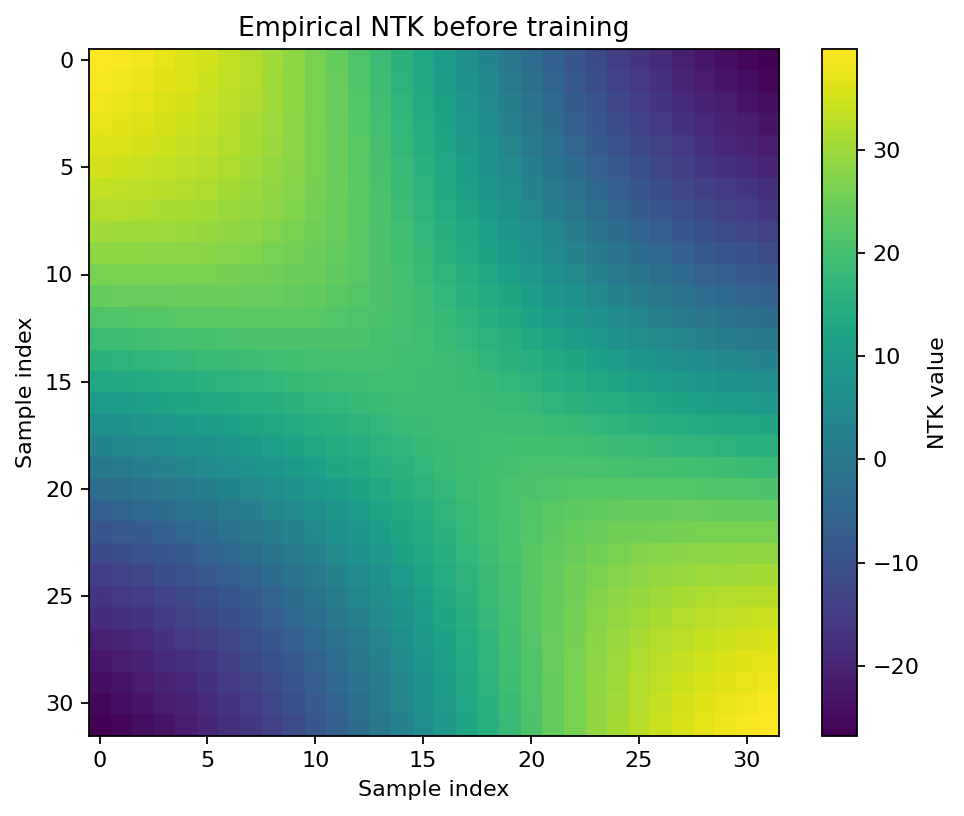
\includegraphics[width=0.72\textwidthы]{../ntk_report_assets/ntk_heatmap_before.png}
    \caption{Эмпирическая матрица NTK до обучения. Гладкая и сравнительно слабо контрастная структура указывает на то, что попарные взаимодействия между объектами на этом этапе определяются главным образом архитектурой сети и случайной инициализацией параметров.}
    \label{fig:ntk_heatmap_before}
\end{figure}

\begin{figure}[ht!]
    \centering
    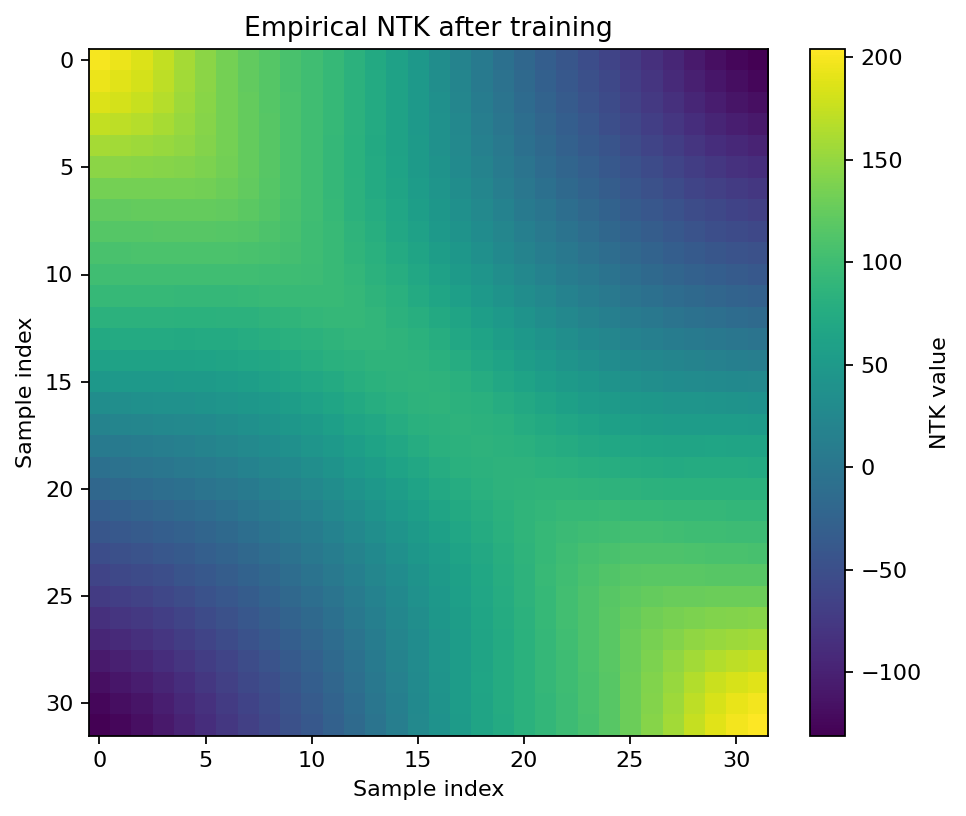
\includegraphics[width=0.72\textwidth]{../ntk_report_assets/ntk_heatmap_after.png}
    \caption{Эмпирическая матрица NTK после обучения MLP на модельной задаче одномерной регрессии. Яркая диагональ отражает сильную чувствительность предсказания в каждой точке к собственным градиентным направлениям, а выраженная вне диагональная структура показывает, что близкие входы оказываются связанными и обучаются не независимо, а согласованно.}
    \label{fig:ntk_heatmap_after}
\end{figure}

Все обсуждаемые ниже визуализации были получены в \texttt{TensorFlow} для одной и той же выборки до и после обучения. На \cref{fig:ntk_heatmap_before} исходное ядро имеет гладкую и менее контрастную структуру: значения матрицы меняются достаточно плавно, а локальная сегментация выражена слабо. Это указывает на то, что на этапе инициализации сеть ещё не сформировала избирательную геометрию взаимодействий между объектами, и соответствующая Gram-матрица отражает прежде всего индуктивное смещение архитектуры.

На \cref{fig:ntk_heatmap_after} структура становится более неоднородной: усиливается диагональ, а вне диагонали проявляются локальные зависимости. Для одномерной регрессии, где соседние индексы соответствуют близким значениям входной переменной, такая картина означает, что обучение усиливает перенос информации между геометрически близкими точками и ослабляет его между более удалёнными областями. Следовательно, индуцированная сетью метрика становится менее изотропной и лучше согласуется со структурой данных.

При чтении тепловых карт NTK следует учитывать, что элемент \(\Theta_{ij}\) характеризует степень согласованности градиентных направлений, соответствующих объектам \(x_i\) и \(x_j\). Яркая диагональ отражает высокую норму собственных градиентных откликов, тогда как интенсивные вне диагональные области указывают на сильную функциональную связь между различными объектами выборки. Если индексы объектов упорядочены в соответствии с геометрией данных, то локальные яркие полосы и блоки естественно интерпретируются как области, внутри которых обновления параметров влияют на предсказания согласованно; напротив, тёмные участки соответствуют слабому переносу информации и относительной декорреляции градиентной структуры.

\begin{figure}[ht!]
    \centering
    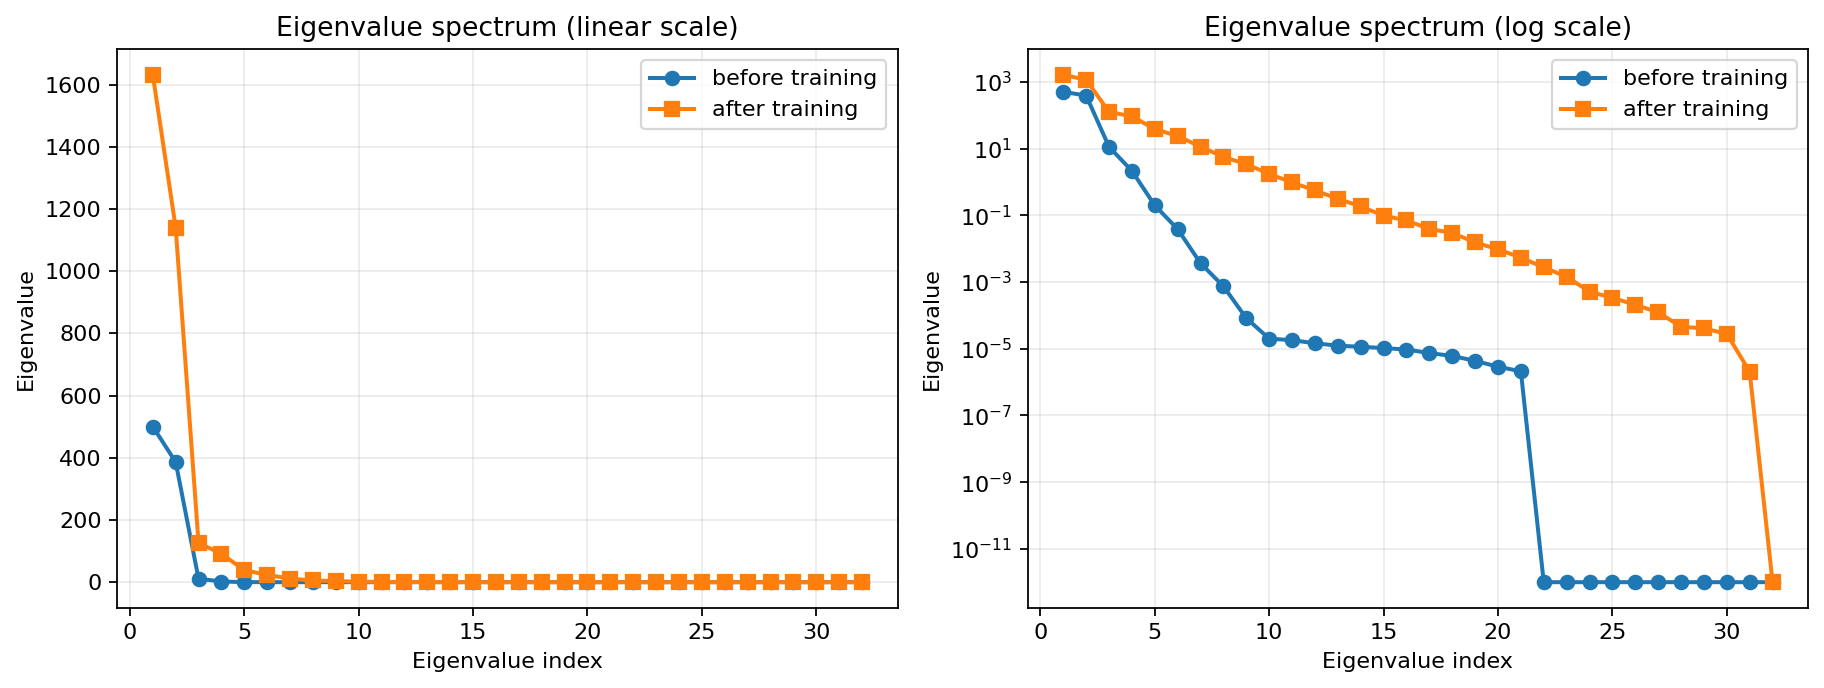
\includegraphics[width=\textwidth]{../ntk_report_assets/ntk_eigenspectrum_before_after.png}
    \caption{Спектр собственных значений NTK до и после обучения. Левая панель показывает спектр в линейном масштабе, правая --- в логарифмическом. После обучения доминирующие собственные значения возрастают, а сам спектр становится более протяжённым, что указывает на увеличение числа направлений в функциональном пространстве, по которым сеть активно адаптируется к данным.}
    \label{fig:ntk_spectrum}
\end{figure}

Из \cref{fig:ntk_spectrum} следует, что после обучения ведущие собственные значения увеличиваются, а спектр спадает медленнее. Это означает, что сеть усиливает чувствительность к нескольким главным направлениям данных и одновременно начинает использовать большее число мод обучения. Если же спектр спадает чрезвычайно быстро, это обычно указывает на близость ядра к низкоранговому и на ограниченную функциональную выразительность на рассматриваемой выборке.

\begin{figure}[ht!]
    \centering
    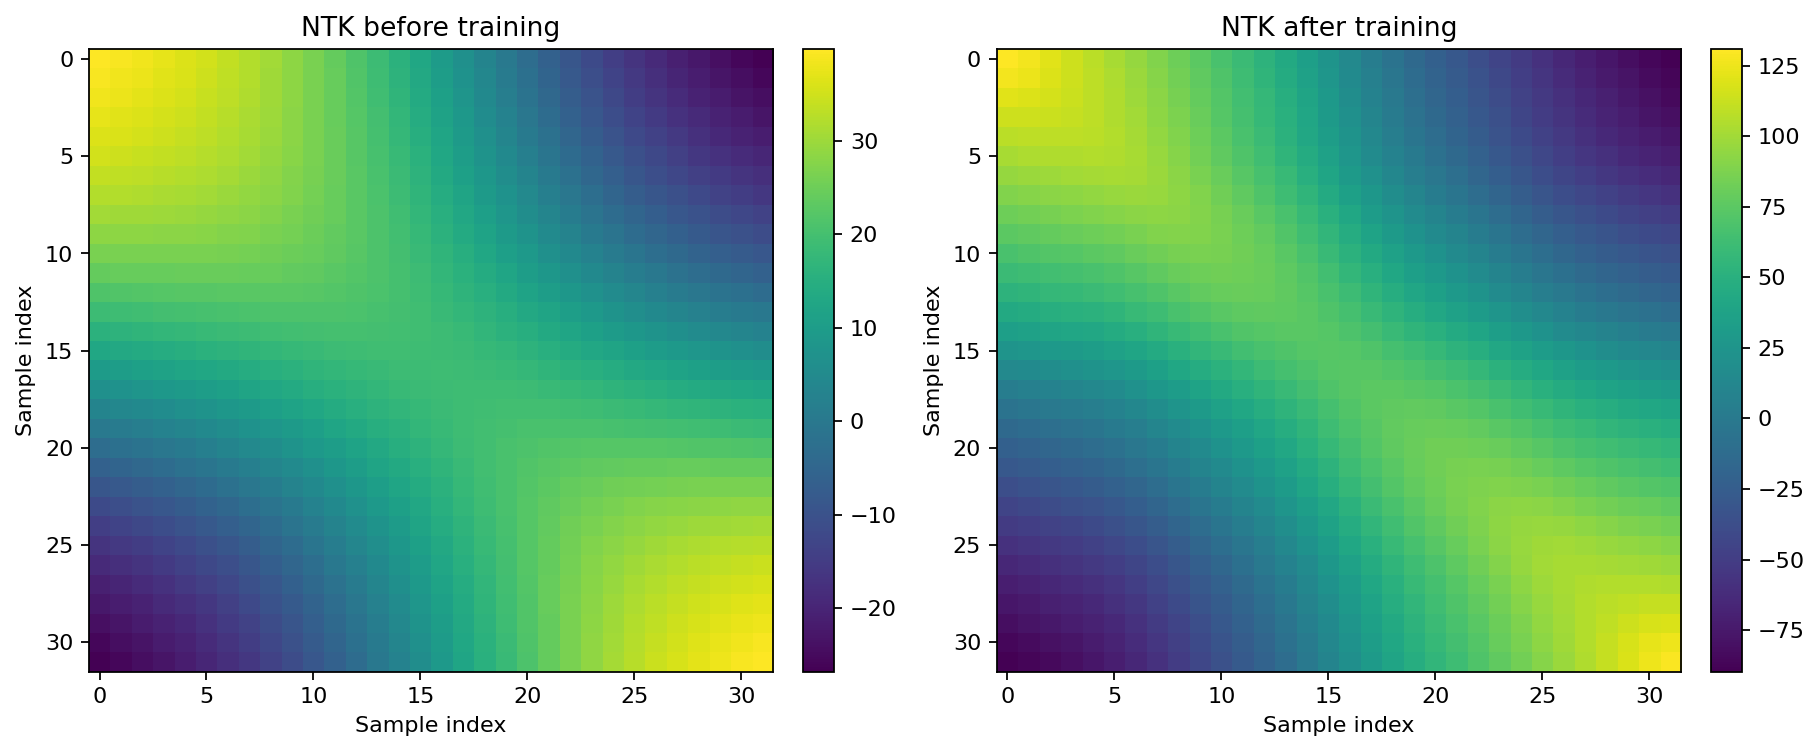
\includegraphics[width=\textwidth]{../ntk_report_assets/ntk_heatmaps_before_after.png}
    \caption{Сравнение матриц NTK до и после обучения. До обучения ядро определяется в основном архитектурой и случайной инициализацией; после обучения структура NTK становится более контрастной, что отражает перераспределение чувствительности модели в соответствии с геометрией данных и целевой функцией.}
    \label{fig:ntk_compare}
\end{figure}

\Cref{fig:ntk_compare} показывает, что глобальная организация ядра сохраняется, однако его локальная структура после обучения становится существенно более выраженной. Иными словами, обучение не разрушает полностью исходное ядровое представление, а перераспределяет веса взаимодействий, повышая разрешающую способность NTK в тех областях, которые значимы для аппроксимации целевой зависимости. Это согласуется с тем, что для конечной ширины сеть не обязана строго оставаться в режиме постоянного ядра: NTK может эволюционировать, и именно эта эволюция отражает частичную адаптацию признакового пространства.

\begin{figure}[ht!]
    \centering
    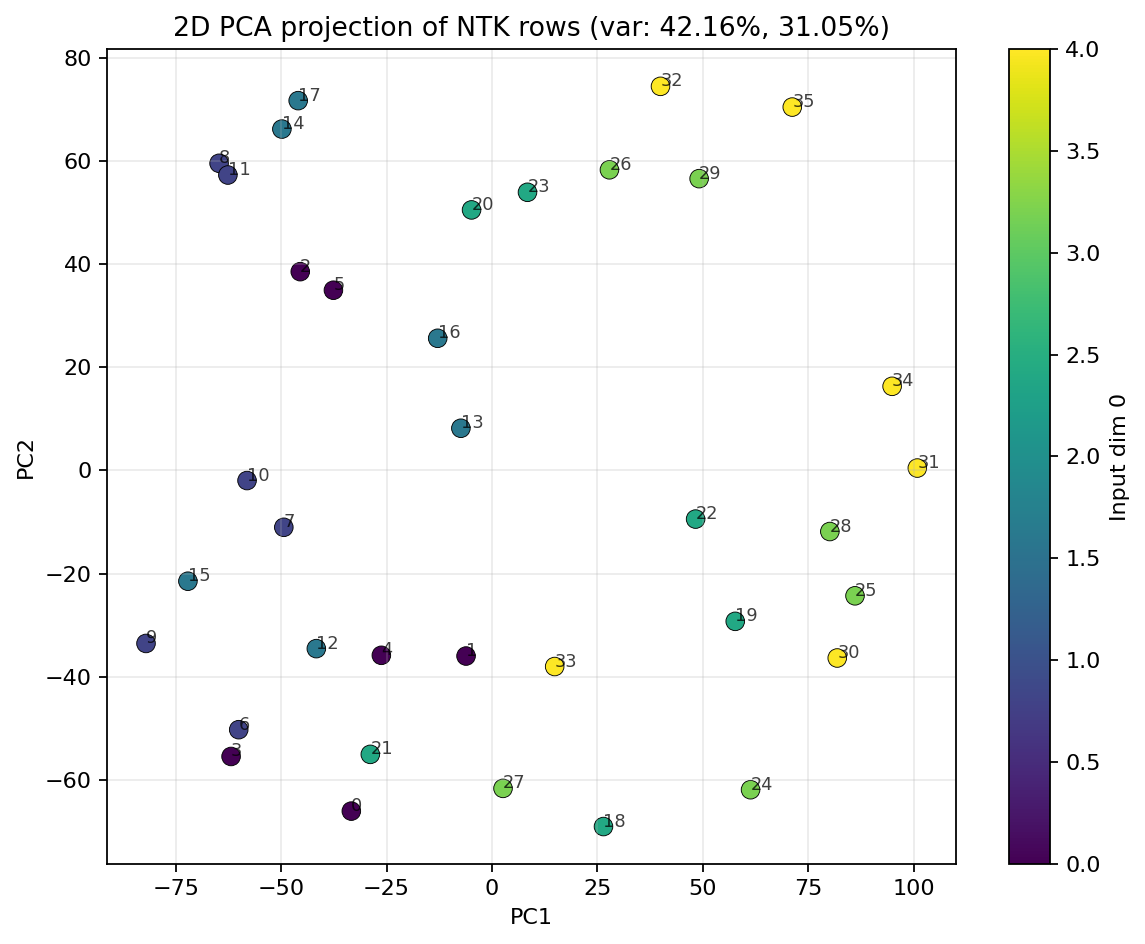
\includegraphics[width=0.8\textwidth]{../ntk_analysis_output_full_model/ntk_rows_pca.png}
    \caption{PCA-проекция строк матрицы NTK. Каждая точка соответствует строке Gram-матрицы, то есть профилю взаимодействия одного объекта со всей выборкой. Пространственное разделение точек отражает неоднородность геометрии данных в индуцированном ядром представлении.}
    \label{fig:ntk_rows_pca}
\end{figure}

PCA-проекция строк NTK на \cref{fig:ntk_rows_pca} позволяет перейти от матричного представления к геометрической интерпретации. Поскольку каждая строка матрицы задаёт вектор сходства одного объекта со всеми остальными, компактные группы точек на плоскости главных компонент соответствуют объектам с близкими паттернами взаимодействия. Напротив, заметный разброс или наличие промежуточных точек указывает на переходные области, где локальная геометрия данных меняется непрерывно, а принадлежность к одной структурной группе не является жёсткой.

\begin{figure}[ht!]
    \centering
    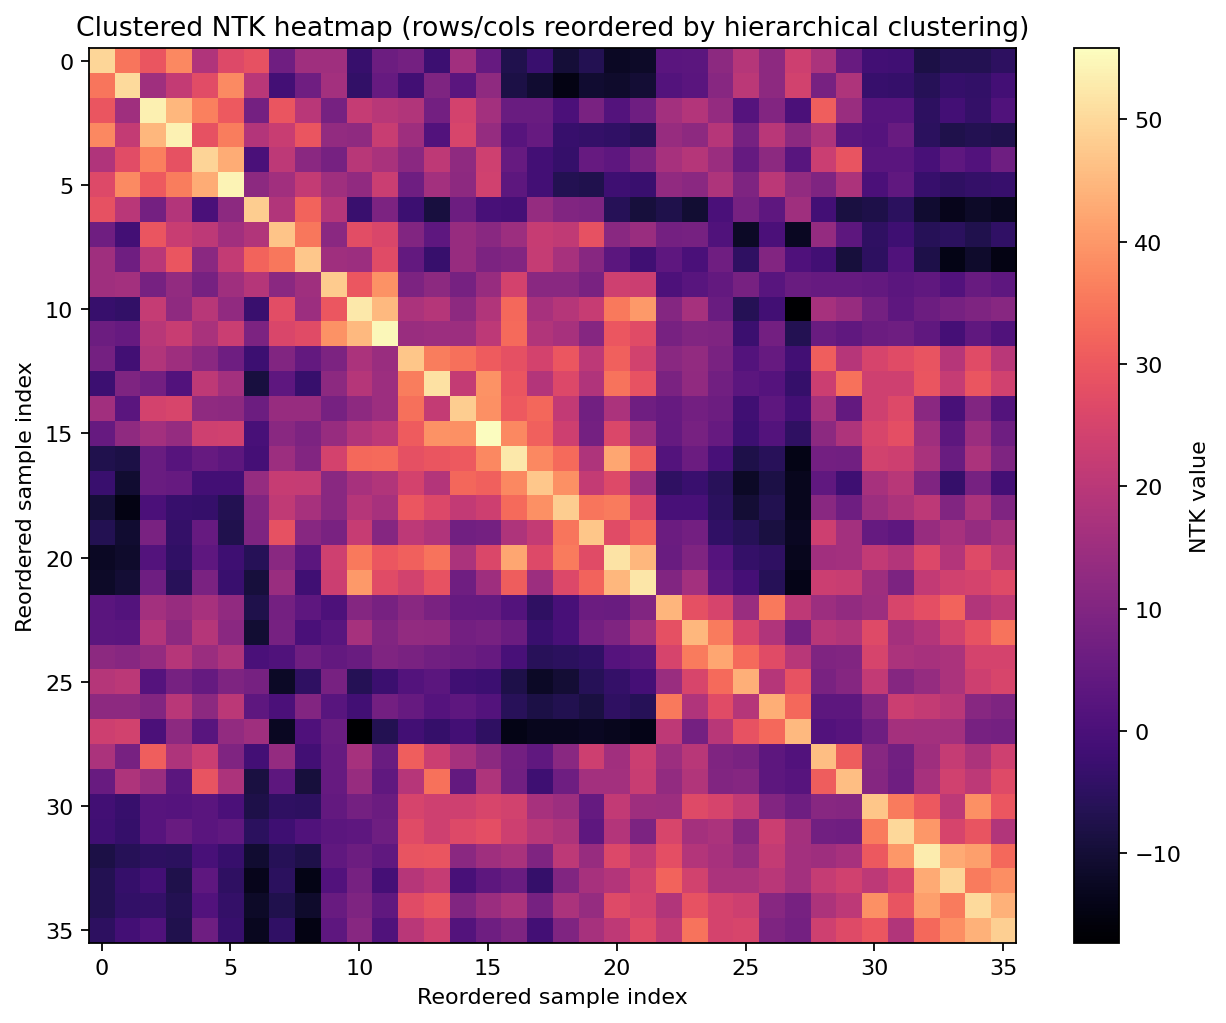
\includegraphics[width=0.85\textwidth]{../ntk_analysis_output_full_model/ntk_clustered_heatmap.png}
    \caption{Кластеризованная матрица NTK. Перестановка строк и столбцов в соответствии с иерархической кластеризацией выявляет блоки объектов с близкими профилями попарных взаимодействий.}
    \label{fig:ntk_clustered}
\end{figure}

Кластеризованная матрица на \cref{fig:ntk_clustered} подтверждает этот вывод: после перестановки строк и столбцов становятся заметны группы объектов, внутри которых значения ядра выше, чем между группами. Такая блочная структура показывает, что данные не образуют однородное облако точек в индуцированном функциональном пространстве. Вместо этого в них присутствуют подмножества с близкой градиентной геометрией, а ненулевые межкластерные связи указывают на существование плавных переходов между этими подмножествами.

\begin{figure}[ht!]
    \centering
    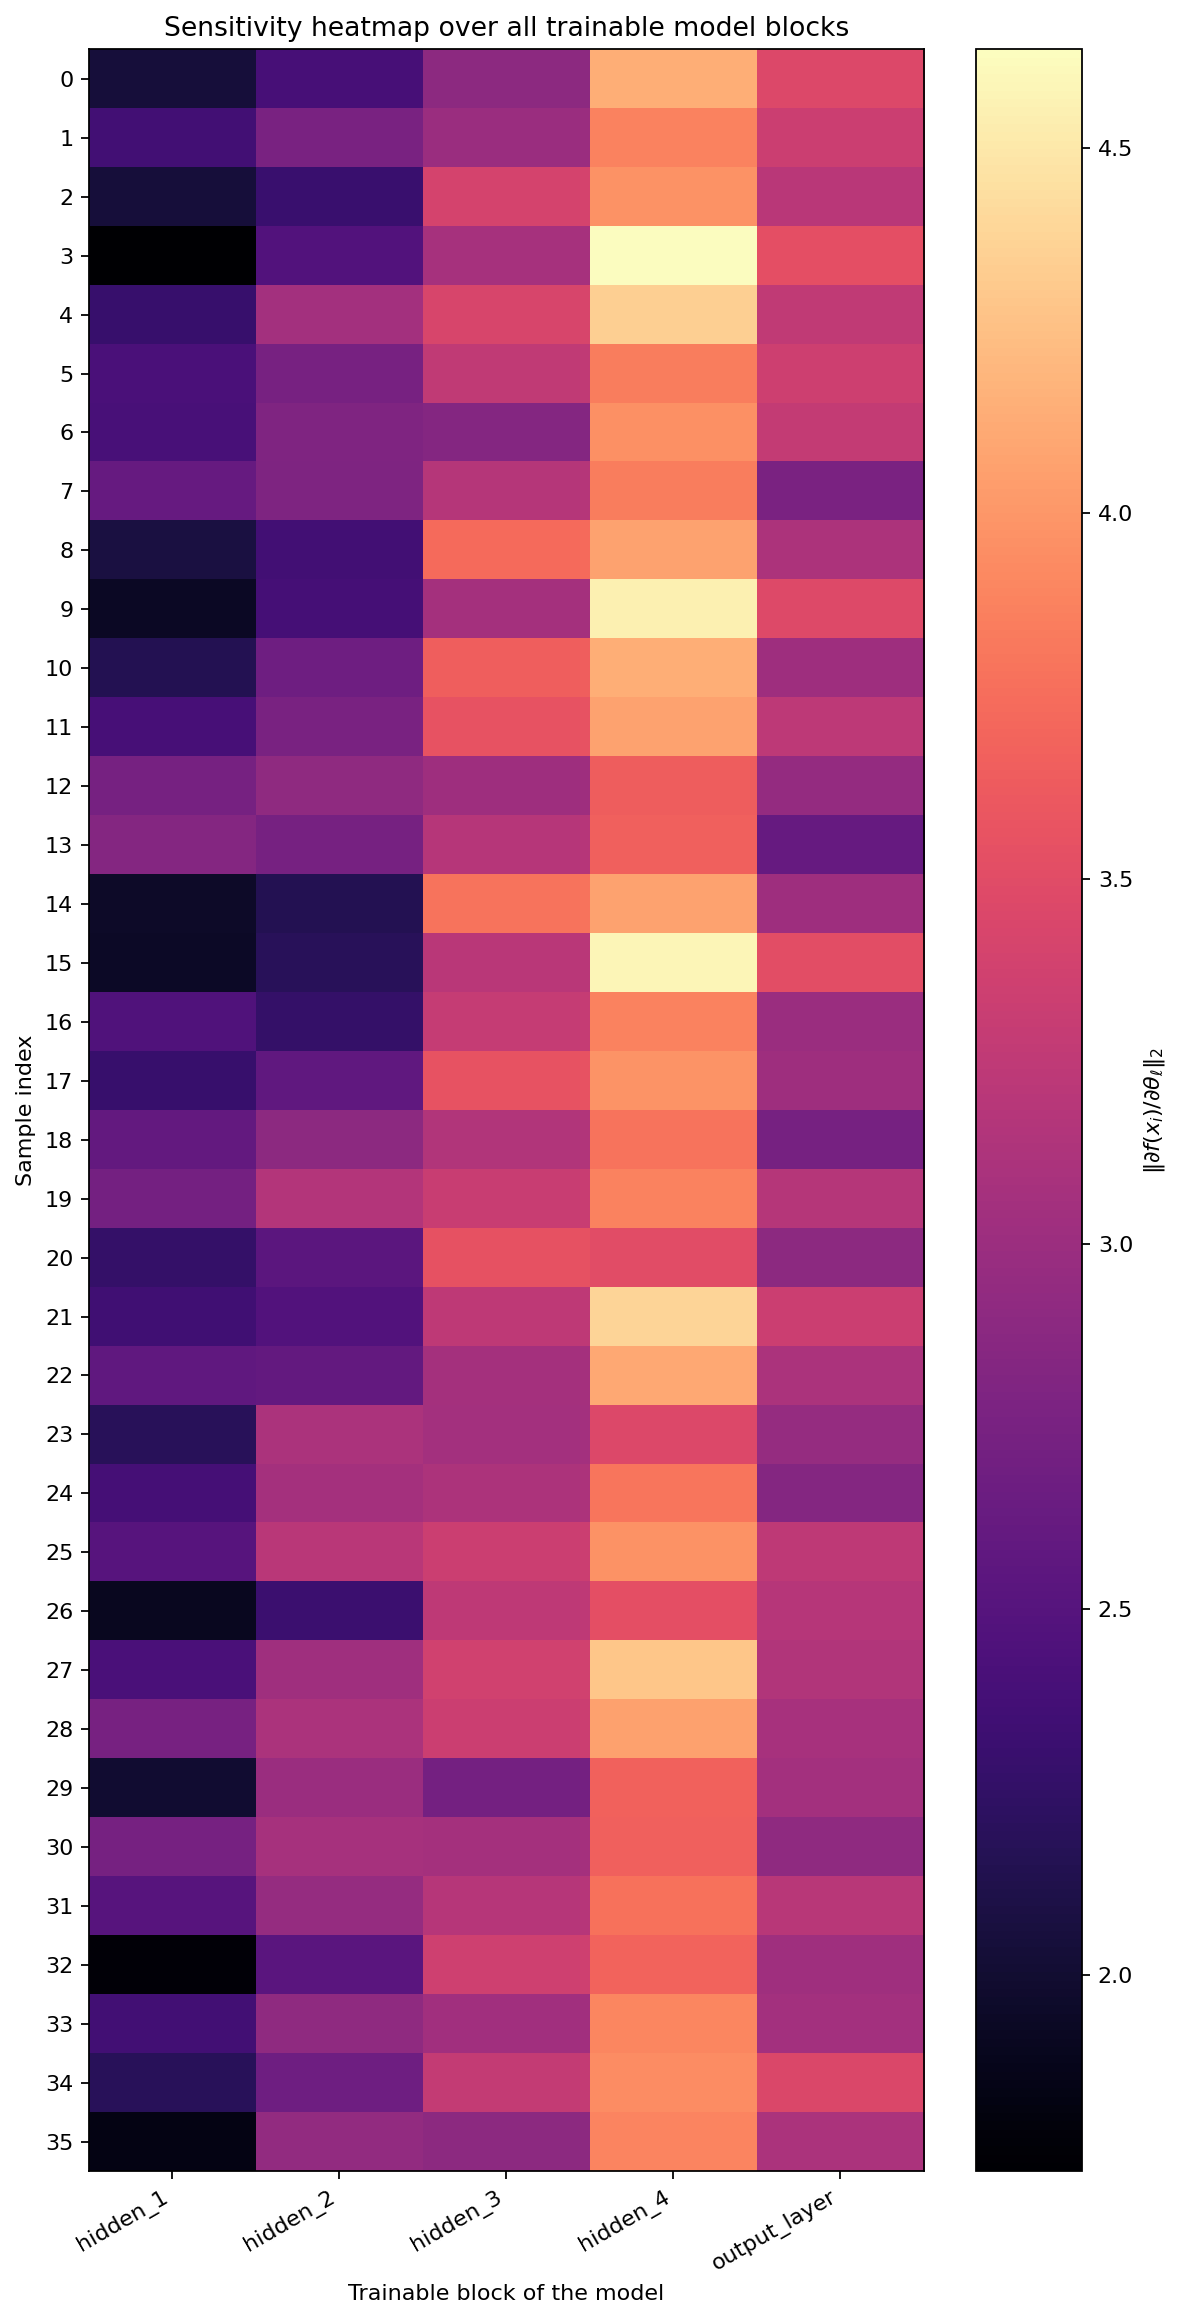
\includegraphics[width=0.86\textwidth,height=0.72\textheight,keepaspectratio]{../ntk_analysis_output_full_model/ntk_model_block_heatmap.png}
    \caption{Карта чувствительности всех обучаемых блоков модели. По строкам отложены объекты батча, по столбцам --- обучаемые блоки сети, а цвет кодирует величину \(\|\partial f(x_i)/\partial \theta_{\ell}\|_2\), то есть вклад соответствующего блока параметров в локальную градиентную чувствительность модели.}
    \label{fig:ntk_model_blocks}
\end{figure}

\Cref{fig:ntk_model_blocks} дополняет попарные тепловые карты NTK и показывает, как в построении ядра участвует вся обучаемая часть модели. В отличие от стандартной матрицы \(\Theta\), где по обеим осям отложены объекты выборки, здесь строки соответствуют отдельным входам, а столбцы --- обучаемым блокам сети. Тем самым визуализация позволяет перейти от вопроса о том, какие объекты взаимодействуют между собой, к вопросу о том, какие части модели ответственны за формирование этих взаимодействий. Светлые вертикальные области указывают на блоки, которые в среднем вносят более существенный вклад в градиентную чувствительность, тогда как горизонтальные контрасты позволяют выделить объекты, для которых распределение чувствительности по слоям заметно отличается от среднего.

Такую карту следует читать по двум направлениям. Сравнение элементов внутри одной строки показывает, какие обучаемые блоки доминируют в отклике модели на фиксированный объект, а сравнение внутри одного столбца характеризует, насколько однородно данный блок реагирует на всю выборку. Если столбец остаётся ярким почти для всех объектов, соответствующий слой вносит устойчивый глобальный вклад в NTK. Если же высокая интенсивность локализована лишь на части строк, это свидетельствует о более избирательной адаптации слоя к отдельным областям входного пространства. Поскольку NTK определяется производными по обучаемым параметрам, в данной визуализации учитываются именно обучаемые блоки сети; фиксированные преобразования входа не образуют самостоятельных столбцов, но косвенно влияют на распределение чувствительности через представление данных на входе последующих слоёв.

\subsection{Интерпретация результатов}

Полученные результаты согласуются с общей теорией NTK. Поскольку матрица ядра определяет функциональную динамику обучения, а в режиме почти постоянного ядра приводит к представлению через kernel regression, анализ её структуры позволяет судить о том, каким образом ошибка в одной точке переносится на остальные объекты выборки. В рассматриваемом примере этот перенос носит не глобально-однородный, а локально-структурированный характер: после обучения влияние обновлений концентрируется в окрестностях геометрически близких точек, что непосредственно видно по усилению диагонали и локальных блоков на тепловых картах.

Спектральные характеристики подтверждают ту же тенденцию. После обучения ранг матрицы возрастает с \(7\) до \(20\), а effective rank --- с \(2.14\) до \(2.95\), что указывает на расширение числа функциональных направлений, в которых сеть действительно адаптируется к данным. Одновременно увеличиваются ведущие собственные значения, поэтому наиболее информативные моды осваиваются быстрее. Такая перестройка спектра хорошо согласуется с PCA-проекцией строк NTK и кластеризованной матрицей: в обоих случаях наблюдается не случайный разброс, а выделение групп объектов со сходными профилями взаимодействия.

Вместе с тем более богатая структура ядра сопровождается ухудшением обусловленности. Condition number возрастает приблизительно с \(2.39 \cdot 10^{8}\) до \(7.94 \cdot 10^{8}\), что указывает на сильную чувствительность малых спектральных мод к численным возмущениям. С практической точки зрения это означает, что доминирующие направления обучения остаются хорошо различимыми, однако хвост спектра оказывается близким к вырожденному. В терминах ядровой регрессии это делает обращение Gram-матрицы менее устойчивым и показывает, что интерпретацию малых собственных значений следует проводить с осторожностью; небольшие отрицательные значения в численном спектре здесь естественно трактуются как артефакты конечной точности вычислений, а не как нарушение положительной полуопределённости NTK.

Дополнительная карта чувствительности по обучаемым блокам модели уточняет этот вывод на уровне внутренней организации сети. Если значимая часть вклада в \(\Theta\) сосредоточена лишь в небольшом числе столбцов, то фактическая адаптация распределяется по модели неравномерно, а спектральная структура ядра в существенной мере определяется ограниченным числом параметрических подсистем. Более равномерное распределение яркости по столбцам, напротив, указывает на то, что формирование NTK опирается на согласованную работу нескольких слоёв. Таким образом, совместный анализ стандартной NTK-матрицы и карты по блокам модели позволяет различать геометрию межобъектных взаимодействий и внутреннее распределение чувствительности по параметрическому пространству сети.
 зрения обобщающей способности важна не только величина ошибки на обучающей выборке, но и то, насколько структура NTK согласована с геометрией данных. Если полезный сигнал проектируется на ведущие собственные векторы ядра, сеть обучается быстрее и переносит информацию преимущественно между действительно близкими объектами, а не между произвольными точками. В рассматриваемом случае усиление локальных зависимостей и появление кластеров в пространстве строк NTK указывают на более содержательное согласование ядра со структурой выборки, что в целом благоприятно для обобщения, хотя высокая обусловленность ограничивает устойчивость по слабым модам.

Наконец, наблюдаемая эволюция NTK позволяет сопоставить результаты с режимами lazy training и feature learning. Если бы обучение происходило строго в режиме lazy training, матрица ядра оставалась бы почти неизменной, а различия между тепловыми картами до и после обучения были бы минимальны. В данном случае глобальная организация NTK действительно сохраняется, однако усиление диагонали, рост эффективного ранга, появление более отчётливых локальных блоков и разделение строк в PCA-пространстве свидетельствуют о нетривиальной перестройке представления. Следовательно, исследуемая сеть работает в промежуточном режиме: ядровое описание остаётся информативным, но обучение не сводится к полностью фиксированному NTK и сопровождается частичной адаптацией признаков.

\subsection{Выводы по разделу}

NTK даёт строгий математический язык для описания обучения нейронных сетей в терминах ядровых методов. Он определяется через градиенты выхода по параметрам, задаёт линейную динамику обучения в режиме почти постоянного ядра и связывает широкие нейронные сети с kernel regression. Анализ спектра NTK, его ранга, effective rank и condition number позволяет судить о качестве индуцированного ядра, о скорости обучения различных мод и о том, насколько архитектура сети согласована со структурой данных. В этом смысле NTK является не только теоретическим объектом, но и практическим инструментом анализа динамики и обобщающей способности нейросетевых моделей.

\newpage
\printbibliography[title={Список литературы }]

\end{document}
